
\documentclass{article}

\usepackage{hyperref}
\usepackage{tabularx}
\usepackage{gantt}
\usepackage{listings}
\usepackage{color}
\usepackage{float}
\usepackage{subfig}
\usepackage[framemethod=tikz]{mdframed}

\hypersetup{
    colorlinks=true, %set true if you want colored links
    linktoc=all,     %set to all if you want both sections and subsections linked
    linkcolor=black,  %choose some color if you want links to stand out
}
\title{EPQ Writeup}
\date{}
\author{James Rand}

\def\tightlist{}

\makeatletter
\def\@seccntformat#1{%
    \expandafter\ifx\csname c@#1\endcsname\c@section\else
    \csname the#1\endcsname\quad
\fi}
\makeatother


\definecolor{mygreen}{rgb}{0,0.6,0}
\definecolor{mygray}{rgb}{0.5,0.5,0.5}
\definecolor{mymauve}{rgb}{0.58,0,0.82}

\lstset{ %
    backgroundcolor=\color{white},   % choose the background color; you must add \usepackage{color} or \usepackage{xcolor}; should come as last argument
    basicstyle=\footnotesize,        % the size of the fonts that are used for the code
    breakatwhitespace=false,         % sets if automatic breaks should only happen at whitespace
    breaklines=true,                 % sets automatic line breaking
    captionpos=b,                    % sets the caption-position to bottom
    commentstyle=\color{mygreen},    % comment style
    deletekeywords={...},            % if you want to delete keywords from the given language
    escapeinside={\%*}{*)},          % if you want to add LaTeX within your code
    extendedchars=true,              % lets you use non-ASCII characters; for 8-bits encodings only, does not work with UTF-8 frame=single,                    % adds a frame around the code keepspaces=true,                 % keeps spaces in text, useful for keeping indentation of code (possibly needs columns=flexible) keywordstyle=\color{blue},       % keyword style language=C,                      % the language of the code
    morekeywords={*,...},            % if you want to add more keywords to the set
    numbers=left,                    % where to put the line-numbers; possible values are (none, left, right)
    numbersep=5pt,                   % how far the line-numbers are from the code
    numberstyle=\tiny\color{mygray}, % the style that is used for the line-numbers
    rulecolor=\color{black},         % if not set, the frame-color may be changed on line-breaks within not-black text (e.g. comments (green here))
    showspaces=false,                % show spaces everywhere adding particular underscores; it overrides 'showstringspaces'
    showstringspaces=false,          % underline spaces within strings only
    showtabs=false,                  % show tabs within strings adding particular underscores
    stepnumber=2,                    % the step between two line-numbers. If it's 1, each line will be numbered
    stringstyle=\color{mymauve},     % string literal style
    tabsize=2,                       % sets default tabsize to 2 spaces
    title=\lstname                   % show the filename of files included with \lstinputlisting; also try caption instead of title
}

\newcommand\mylstcaption{}
\mdfdefinestyle{mymdstyle}{
hidealllines=true,
middleextra={
  \node[anchor=west] at (O|-P)
    {\lstlistingname~\thelstlisting\  (Cont.):~\mylstcaption};},
secondextra={
  \node[anchor=west] at (O|-P)
    {\lstlistingname~\thelstlisting\  (Cont.):~\mylstcaption};},
splittopskip=2\baselineskip
}
\surroundwithmdframed[style=mymdstyle]{lstlisting}
\newmdenv[style=mymdstyle]{mdlisting}

\begin{document}


\maketitle

\tableofcontents
\setcounter{tocdepth}{5}

\newpage

\section{Introduction}
\subsection{Objective}

In this extended project I plan to design a device that will be able to interact with a file
server. This device must be able to acheive some of the following functions:

\begin{itemize}
    \item Be able to turn the server on and off
    \item Be power efficient so the running cost is low
    \item forward a shell connection onto the server
    \item Have an interface to interact with the device
    \item Do not exceed the budget of \$50
\end{itemize}

The first object that I wish to discuss is having the ability to remotely turn on and off the
server. This could be done in two ways: the first would be to use wake on lan which would be
a way of doing it through software; the second is using electrical components to act as an
electric switch. \\

The first approach I would like to talk about is using wake on lan. This seems to be the default
way of doing what I am proposing which means that setting this up will be straight forward and
well documented. The only problem with using this method is that the server will constantly need
to be on standby which conflicts with my second goal of this project being power efficient. The
second approach is the opposite of the first as it will be more difficult to set up due to the
fact it will require me to buy parts which need to be appopiate to interact the server. On the
plus side though it could be a more power efficient as I could design it to control the mains
power supply as well so that it will not need to be on standby.

\subsection{Time scale}

Since I have a limited amount of time to acheive my goal I have created the following Gante
chart (Fig ~\ref{fig:Gantt Chart}) to illustrate how I intend to use my time. This chart
only shows how I will use the time up to the initial draft. There is time availiable after
this draft but I would like to use this time to improve my write up and act upon feedback.

\begin{figure}
    \begin{gantt}[xunitlength=\textwidth / 16]{7}{16}
        \begin{ganttitle}
            \titleelement{Number of weeks}{16}
        \end{ganttitle}
        \begin{ganttitle}
            \numtitle{1}{1}{16}{1}
        \end{ganttitle}
        \ganttbar{Research}{0}{7}
        \ganttbarcon{Design}{7}{2}
        \ganttbarcon{Building}{9}{4}
        \ganttbarcon{Reflection}{13}{3}
        \ganttmilestone[color=cyan]{Draft deadline}{16}
        %\ganttmilestonecon{A connected Milestone}{7}
    \end{gantt}
    \caption{Gantt chart} \label{fig:Gantt Chart}
\end{figure}

\break
\section{Reseach}
\subsection{choosing the right board}

The very first thing that I need to consider when designing this is what development board
I will as everything else will be dependant upon this. The 4 factors that I decided would
be most important to consider are: the price of the board; how easy it would to connect
and control through the internet and power consumption.

The reason I think power consumption should be something to consider is that this board will
be on for long periods of time to make sure that the server is always available. Which means
running a power hungry device will be expensive and not pratical. The price is an obvious
important feature and since I may be buying extra hardware components I need to be extra wary of
the cost of the board. Since I will be controlling the board through the internet it needs to
have internet connectivity and be straightforward to setup. Finally I need to think about the
implications of the hardware. This means the board must be able to communicate to hardware from
a custom written program.

\subsubsection{Raspberry Pi}

The Raspberry Pi is definatly one of the more well known development boards that are use
extensively by hobbyists. This means that the Raspberry Pi will be well documented so if
I come across any difficulties it will be easier to troubleshoot. The table below compares
the technical specs of all of the models. \\

\begin{tabularx}{\textwidth}{| X | X | X | X | X |}
    \hline
    Raspberry Pi Model & Model A+ & Model B & Model B+ & Model B 2 \\ \hline
    Price              &  \$19.99  &  \$39.99 &  \$29.99  &  \$39.99   \\ \hline
    Processor Speed    &  \multicolumn{4}{c |}{700 Mhz}  \\ \hline
    Power Consumption  &  \multicolumn{3}{c |}{600mA @ 5V} & 650mA @ 5V \\ \hline
    Memory             &  256MB   & \multicolumn{2}{c |}{512MB} & 1GB \\ \hline
    Storage            &  Micro SD Card &  SD Card & \multicolumn{2}{c |}{Micro SD Card} \\ \hline
    Pins               &  40      &    26  & \multicolumn{2}{c |}{40} \\ \hline
    Coding Languages   &  \multicolumn{4}{c |}{Python} \\ \hline
\end{tabularx}
\newline

The source of the information is in the refrences\cite{raspberryPi}
\newline

The characteristics that I have mentioned above make the raspberry effortless to develop on;
mainly because it runs the linux operating system. This means that I can use and run any language
that runs linux givving me a wide range of tools to use. I could also install and use programs that
other people have written. As mention above the raspberry pi is very popular meaning the is a wide
range of hardware extenstion that may make it easier to control external components.

\subsubsection{BeagleBone Black / BeagleBone Black Wireless}

This section will cover a comparison of features on the BeagleBone Black and the BeagleBone Black Wireless.
The only difference between these boards is that one has bluetooth and wifi while the other has ethernet.
These boards, similar to the raspberry pi, are very popular meaning there is a wide range of documentaion
and addons that can be used although it should be noted that they are not as popular as the raspberry pi.
The table below will give a summery of the features availiable. \\

%\newline
\begin{tabularx}{\textwidth}{| X | X | X |}
    \hline
    BeagleBone Model &  BeagleBone Black  & BeagleBone Black Wireless \\ \hline
    Price            &       \$75         &        \$80               \\ \hline
    Processor Speed  &  \multicolumn{2}{c |}{1GHz}                    \\ \hline
    Power Consumption&  \multicolumn{2}{c |}{210-460mA @ 5V}          \\ \hline
    Memory           &  \multicolumn{2}{c |}{512MB}                   \\ \hline
    Storage          &  \multicolumn{2}{c |}{2GB eMMC}                \\ \hline
    Pins             &  \multicolumn{2}{c |}{2x46 pin headers}        \\ \hline
    Coding Languages &  \multicolumn{2}{c |}{C/C}                   \\ \hline
\end{tabularx}
\newline

The source of the information is in the refrences\cite{beagleboard}
\newline

The first thing that I noticed when researching this board is that it can be pricey but looking
at the specs you can see why. These boards are very similar to the raspberry pi but I thought it
was worth discussing this board as it excels in hardware thanks to it's many pins. Simarly to the
raspberry pi it also runs Linux. The BeagleBone also has lower power consumption than the raspberry
pi. Finally it is worth noting that it uses C/C++ for the programming language which is more difficult
to write in than a language such as Python.

\subsubsection{Audino Uno}

The Audino is a classic development board that instead of the previous two items does not have the linux
operating system. That being said due to it's large poplarity there are a huge number of libraries and
APIs that you can use. \\

\begin{tabularx}{\textwidth}{| X | X |}
    \hline
    Audiono Model    &   Audiono Uno \\ \hline
    Price            &       \$25    \\ \hline
    Processor Speed  &      16MHz    \\ \hline
    Power Consumption&    50mA @ 5v  \\ \hline
    Memory           &      32KB     \\ \hline
    Pins             &       20      \\ \hline
    Coding Languages &     C/C++     \\ \hline
\end{tabularx}
\newline

The source of the information is in the refrences\cite{ardino}
\newline

The specs on the ardunio are considerably lower than the previous two items due to the fact that
the arduino is a microcontroller instead of a size down computer. This means that it consumes less
power and has less features that the other two can offer. There is also a problem with wireless
capabilities on the audino as it has none built in and would require me to buy a WiFi sheild.

\subsubsection{Particle Photon}

This board is much more obscure than the rest of the boards that I have compared. Despite this there
are a lot of attractive charactersitics that this board like the fact that it has in built wireless
and can be communicated with through the internet without the need to port forward. Additionaly this
board is the smallest of all of the ones that I have considered. \\

\begin{tabularx}{\textwidth}{| X | X |}
    \hline
    Particle Model   &    Photon     \\ \hline
    Price            &     \$19      \\ \hline
    Processor Speed  &    120Mhz     \\ \hline
    Power Consumption& 80mA @ 5V-3.3V\\ \hline
    Memory           &    128KB      \\ \hline
    Storage          &     1MB       \\ \hline
    Pins             &     28        \\ \hline
    Coding Languages &    C/C++      \\ \hline
\end{tabularx}
\newline

The source of the information is in the refrences\cite{particlePhotonSpec}
\newline

Similarly to the Arduino this board is a microcontroller. The features I mentioned above reagarding
connectivity will make development considerable easier. This is also the cheapest board that I have
compared giving me plenty of left over money to buy all the hardware components that I might need.


\subsubsection{The Board I Chose}

After considering the pros and cons of all of these boards I decided that a microcontroller type
would be much more suitable for my project. My reasoning behind this is that a fast processor and
a linux operating system is unecessary in this situation meaning that I would be wasting power on
features that I am not going to use. The price is also higher for the non-microcontrollers.

I now needed to make a decision between the Audino and the Particle Photon. Although the arduino has
a huge number of libraires and a comprehensive documentation; I came to the conclus

\subsection{Transitors vs Relays}

In order to interact with the server on a hardware level I need a component that can act like an
electrical switch. This is so that when I need to turn the server on and off I can acheive this with
this "electical switch". There are two components that took my interest while researching this. The
first is transitros which are part of the semiconductor family and are largely used in computers. The
second is a relay which unlike a transitor has moving parts and works using an electro magnet. The first
that I will discuss in detail are transitors.

\subsubsection{Transitors}

\begin{figure}
    There are many different types of transistors but the most common and the one I am most interested in is
    the "Bipolar junction transistor" or "BJT" for short. There are two types of BJT that I need to discuss
    which are NPN and PNP. Before I start describing those it is importatnt to understand the basic anotomey
    of transistors first.

    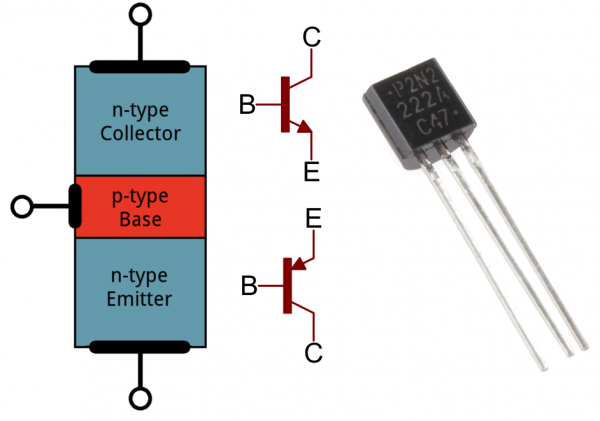
\includegraphics{pictures/transistor-layout.png}
    \caption{transistor layout} \label{fig:transistor-layout}
    \vspace{0.5cm}

    In the layout above (Fig ~\ref{fig:transistor-layout}) you can clearly see that a transitor has three legs.
    These legs each do different things and have special names: collecter, base and emitter. The leg in the middle
    called the base is the one we are most interested in as this can control the current throught the emitter and
    collector by varying the input to it. The collector and emitter can change based upon the type of transitor

\end{figure}

\begin{figure}
    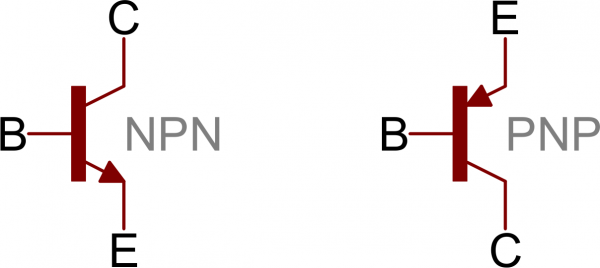
\includegraphics{pictures/npn-pnp-symbols.png}
    \caption{NPN vs PNP} \label{fig:different-transitor-layout}
    \vspace{0.5cm}

    The two different diagrams above show the different types of BJT transitors
    (Fig ~\ref{fig:different-transitor-layout}). \\

    The only difference between these two types which is illustrated by this figure is the direction of the
    emiiter arrow. This small difference has big implications and lead to different properties for each. I
    will now start to disscuss these consequences and which out of the two I think is most suitable for this
    project.

\end{figure}

\break

Unlike many other electrical components like resistors and capacitors which have a linear relationship with
voltage and current transitors have four different ways of handling electrical power:

\begin{itemize}
    \item Saturation     --- Which freely alows volatage and current to flow from the collector to emitter
    \item Cut-off        --- Allows no volatege or current from collector to emitter. Oposite of "Saturation"
    \item Active         --- The current from the collector to emitter is proportional to the current flowing
        through the base
    \item Reverse-Active --- Similar to "Active" the current is proportional to the base but flows in reverse
\end{itemize}

For the purposes of this project the only modes worth discussing are "Saturation" and "Cut-off" because we
are only interested in on or off and not anything inbetween.

To determine what mode the transistor is in you need to investigate what voltage is supplied to each pin.
In order to put a NPN transistor into staturation mode the volatege supplied to the base, V\textsubscript{B}
needs to be greater that the voltage supplied to the emitter, V\textsubscript{E}. To put into cut-off mode
it needs to be the opposite. Likewise with PNP transistors it is reversed.

After considering these factors I decided to perform an experiment to get use to using transistors. I did
this by connect up an led and transistor to my board and checking that I can turn it off and on by emmitting
an output voltage on one of the pins. A schematic of my experiment can be seen below in figure >>>>>>.



I flash a example program onto the board called "Blinky". The purpose of this program to to turn a output
pin on and off every second. This output pin is labeled the voltage alternator in th diagram. After I
design this circuit I then built it on a bread board which is shown below in figure >>>>>>>. The result
of this is the led turn off and the on again.

The source of the information for this section can be found in the references \cite{transistor}

\subsubsection{Relay}

An alternative to the transistors is the relay. Similarly to the transistor this can work as an electronic
switch. The main difference between a relay and a transistor is that a relay have physical moving parts
inside. Inside a relay there is an electro magnet which can pull a thin piece of metal down to make the
switch close. This is how a relay works. Due to this mechanisism a relay can be significantly bigger than
a transistor and it can calso handle higher volatages with ease. A downside to a relay is that it can
take longer for it to switch on and off. Luckly with my choice of board there is a addon board that has
relay support called the "Relay shield"\cite{relaySheild}. This make setting up the relays significantly easier than setting
up the transistors. This relay sheild can also handle high voltages meaning it may be able to control the
mains supply to the server making it more power efficient than transistors. The only downside to using this
addon is that it is significantly more expensive than using the raw components. A picture of this
addon board is shown down below in figure ~\ref{fig:relayShield}.


\begin{figure}[H]
    \noindent\makebox[\textwidth]{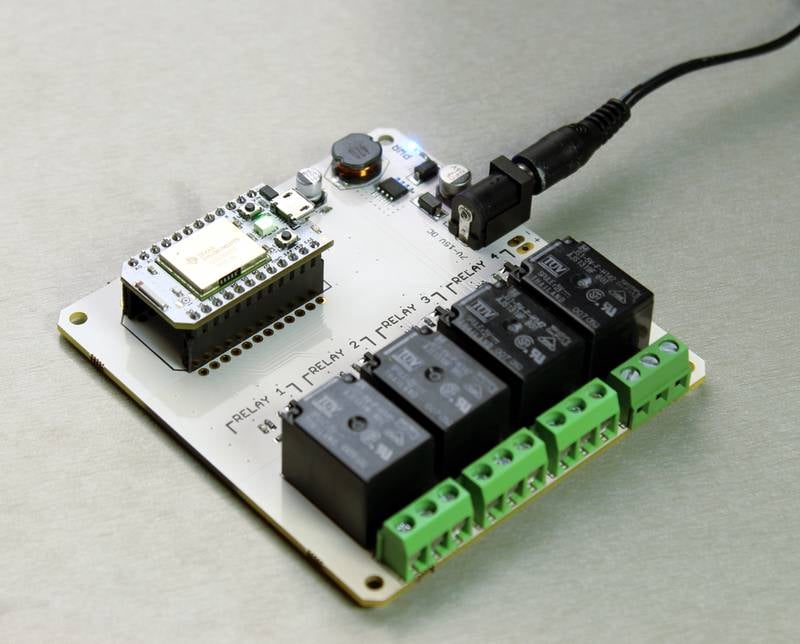
\includegraphics[width=\paperwidth-3cm]{pictures/relay-shield.jpg}};
    \caption{Picture of the relay shield} \label{fig:relayShield}
\end{figure}

\subsubsection{Conclusion}
In conclusion I decided to go with the relay addon board due to it being designed for this exact practice and
it's convience. Even though the experiment performed with the transistor was sucessful it would fail on
higher voltages on the mains therefore it would be less power efficent.

\section{Design}

After doing this research I think it is now time to move on and start building schematics and pesudo code
for how I want the project to look like. I think the most critical component of this project is the
actual functionality of turning the relay on and off remotely.

\subsection{Turning the relay off and on remotely}
I think the first thing I would like to approach would be the software behind this action. My reasoning
behind this is that the hardware setup will be very similar to the relay test hardware the only difference
is instead of having an led I will have the two power wires from the server.

\subsubsection{Software}
Before describing how I plan to turn the server off and on I would like to explain the basic structure of
the particle photon api.

Within the partivle photon api there are three basic functions: setup() and loop(). The first function
setup is run when the particle photon boots up so this should be use to initialize any important variables
that will be used throughout the function. The second procedure loop repeats all of the code inside as long
as the photon is switch on. Below is some example code that was use during the tests for the relay and the
transistor called blinky. This simply turns an pin output on and off and is show in Fig ~\ref{fig:exampleCode}

\begin{figure}
    \begin{lstlisting}

        int led1 = D0; // Instead of writing D0 over and over again, we'll write led1
        int led2 = D7; // Instead of writing D7 over and over again, we'll write led2

        void setup() {

          // We are going to tell our device that D0 and D7 (which we named led1 and led2 respectively) are going to be output
          // (That means that we will be sending voltage to them, rather than monitoring voltage that comes from them)

          // It's important you do this here, inside the setup() function rather than outside it or in the loop function.

          pinMode(led1, OUTPUT);
          pinMode(led2, OUTPUT);

        }

        // Next we have the loop function, the other essential part of a microcontroller program.
        // This routine gets repeated over and over, as quickly as possible and as many times as possible, after the setup function is called.
        // Note: Code that blocks for too long (like more than 5 seconds), can make weird things happen (like dropping the network connection).  The built-in delay function shown below safely interleaves required background activity, so arbitrarily long delays can safely be done if you need them.

        void loop() {
          // To blink the LED, first we'll turn it on...
          digitalWrite(led1, HIGH);
          digitalWrite(led2, HIGH);

          // We'll leave it on for 1 second...
          delay(1000);

          // Then we'll turn it off...
          digitalWrite(led1, LOW);
          digitalWrite(led2, LOW);

          // Wait 1 second...
          delay(1000);

          // And repeat!
        }
    \end{lstlisting}
    \caption{Example Code} \label{fig:ExampleCode}
    \vspace{0.5cm}
    The comment lines denoted by "//" explain what is happening in the code.
\end{figure}

Now that I have explained the basics I can now describe some code that should allow me to turn
a relay on and off. This code is shown in ~\ref{fig:relayTest}.
\begin{figure}
    \begin{lstlisting}
        int relayState = 0;


        void setup()
        {
           //Initilize the relay control pins as output
           pinMode(RELAY1, OUTPUT);
           // Initialize all relays to an OFF state
           digitalWrite(RELAY1, LOW);
           //register the Particle function
           Particle.function("relay", relayControl);
        }

        void loop()
        {
           // This loops for ever
        }

        // command format r1,HIGH
        int relayControl(String command)
        {
          // invert the relay number
            relayState = !relayState;


          // write to the appropriate relay
          digitalWrite(0, relayState);
          return 1;
        }
    \end{lstlisting}
    \caption{Relay Test Code} \label{fig:relayTest}
    \vspace{0.5cm}
    The code is similar to the previous example (Fig ~\ref{fig:ExampleCode}) the only big
    difference in the "relayControl" function. All this function does is turn the relayState
    variable to a one if it is a zero and to a zero if it is a one. Once it has done this it
    set the relay to this new state. In the setup() function I register this function with
    particle which means that I can now trigger this function remotely using a POST request.
\end{figure}

\pagebreak
To trigger this function with a http POST request I needed to know two pieces of information
. The first is my device id which is a number that is assign to every particle photon connect
to the particle cloud. This is use so the particle cloud know what device I want to select.
The second piece of information is my access token. This another number that is assign to
my account instead of the actual device. This enables the particle cloud to verify that I
am who I say I am. Similar to a password.

I can then modify this code to get to be more specific to the turning on the server.

\begin{figure}
    \begin{lstlisting}
    int RELAY1 = D0;

    void setup()
    {
       //Initilize the relay control pins as output
       pinMode(RELAY1, OUTPUT);
       // Initialize all relays to an OFF state
       digitalWrite(RELAY1, LOW);

       //register the Particle function
       Particle.function("relay", relayControl);
    }

    void loop()
    {
       // This loops for ever
    }

    // command format r1,HIGH
    int relayControl(String command)
    {
        digitalWrite(0, 1);
        delay(500);
        digitalWrite(0, 0);

        return 1;
    }
    \end{lstlisting}
    \caption{Relay Code} \label{fig:relayCode}
    \vspace{0.5cm}
    This code turns on the relay for 500 miliseconds and then turns it back on again
    meaning the relayControl function is now used exclusively to turn on the server.
    This is becuase later on I find an interest feature of the server meaing the photon
    will not be turning the server off.

\end{figure}

\subsubsection{The Hardware}
The next thing to design in terms of turning on the server is to look at the hardware.
Fortunatly it is simple to set up and is similar to the hardware in the relay test. The main
part of the hardware are two relays that control mains power supply and turning the server on
from standby and are connected up to the pins "D1" and "D0" respectively. I have also added a
override switch which will block any attempt to turn on the server. There is however a difference
between the relay responsible for the mains power supply and the relay for turning on the server
and that is the inputs that they are connected up to. The mains power suppy is hooked up to the NC
input meaning that current can flow through normally unless the particle photon powers the relay. While
the relay for turning on the server is connected to NO inputer meaning that current can only flow
if the relay is powered. This makes sense as in the next section I talk about automatically turning
off the relay board after it is finished turning on the server meaning that it will not be able to
consistantly power on the relay on the mains.

\begin{figure}[H]
    \noindent\makebox[\textwidth]{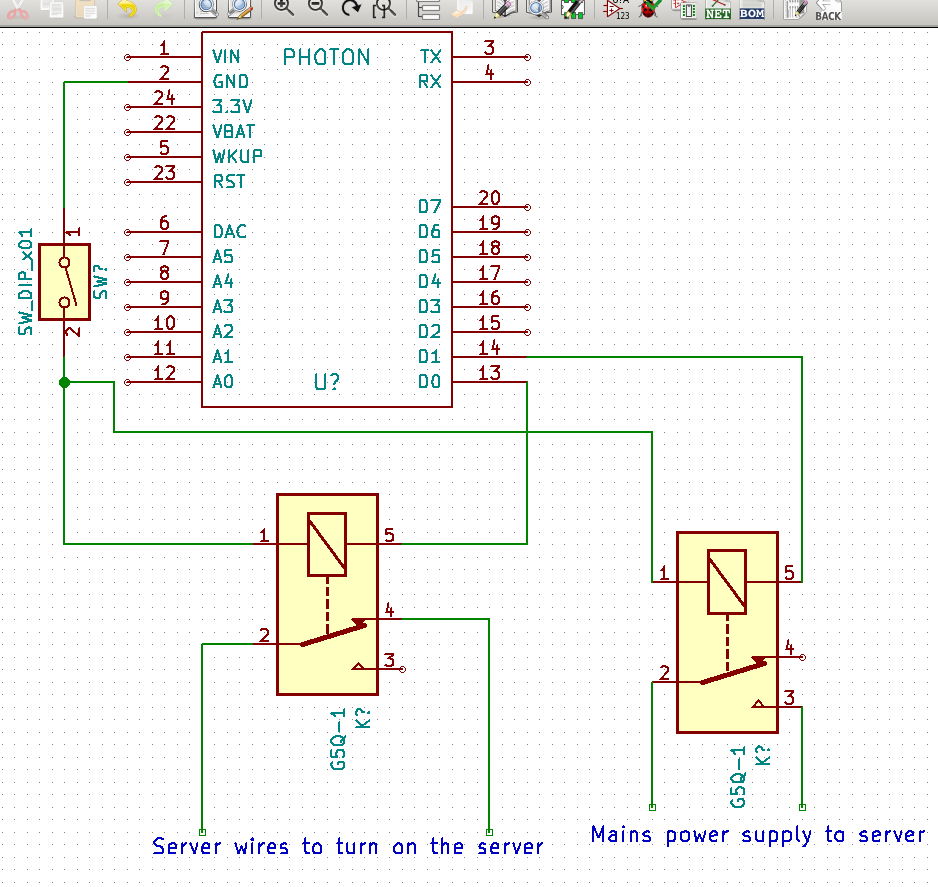
\includegraphics[width=\paperwidth-3cm]{pictures/turnOnRelay.png}};
    \caption{Hardware schematic} \label{fig:turnOnRelay}
\end{figure}


\subsubsection{Taking advantage of a quirk of the server}
Interestly the server exhibits an odd behaviour that I can take advantage of to improve my
project which is that the usb ports are not powered when the server is on standby but is powered
when it is turn on. This is useful for two reasons: the first is that I can use it to properly
check whether the server has successfully turn on and the second is that I can use this new
power to turn off the particle photon board after it has finished turning on the server.

This does have a side affect however. Which is that I can no longer use the particle
photon to turn off the server. This is easily resolved as I plan to have an ssh interface
with the server meaning I turn it off throuh that connection.

This new feature requires me to add to the design of the hardware. Figure ~\ref{fig:usbSch}
essentially outlines what I want to add. It shows a relay hooked up to the power source of
the photon so that it is normally closed. But when power is supplied to this relay from the
usb the relay becomes open turning off the board.

\begin{figure}[H]
    \noindent\makebox[\textwidth]{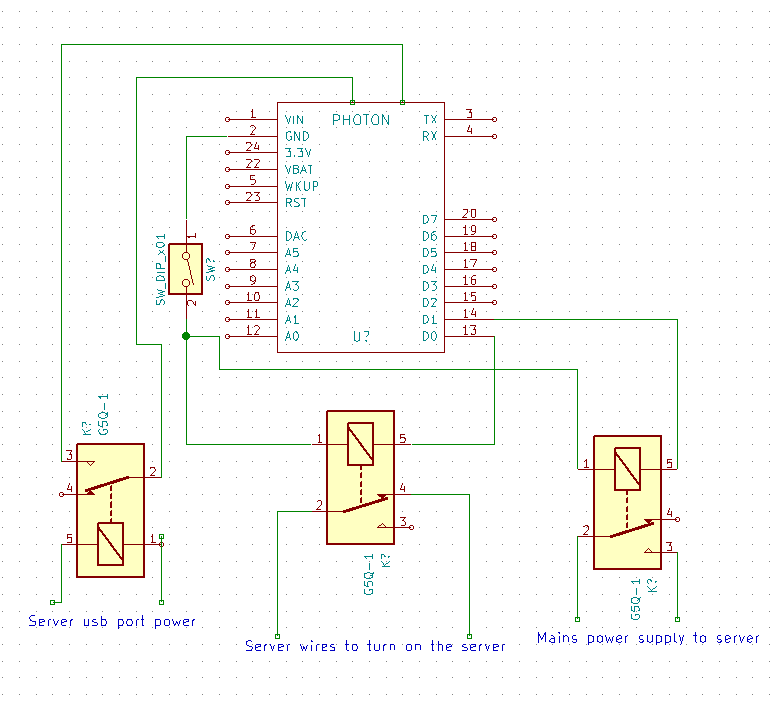
\includegraphics[width=\paperwidth-3cm]{pictures/usbLoopSch.png}};
    \caption{Usb schematic} \label{fig:usbSch}
\end{figure}

\subsection{Forwarding a shell}
Another requirement for device is to be able to forward a shell onto the server. Doing this
purely from this device is counter productive and goes beyond the scope of this project. The
approach that make most sense for this project is to have the particle photon grab the public
ip address and return this to a client whenever the client issues the command to turn on the
server. This client will be the the interface for the device stated in one of the predetermined
goals. For the moment I will analyze what is need to grab the public ip on the deivce. Fortunatly
this can be done using the particle photon api\cite{publicIPDocs}. The example code given by the
documentation is given below in figure
~\ref{fig:publicIpExample}

\begin{figure}[H]
    \begin{lstlisting}
    // Open a serial terminal and see the IP address printed out
    void handler(const char *topic, const char *data) {
        Serial.println("received " + String(topic) + ": " + String(data));
    }

    void setup() {
        Serial.begin(115200);
        Particle.subscribe("particle/device/ip", handler);
        Particle.publish("particle/device/ip");
    }
    \end{lstlisting}
    \caption{Public Ip Example code} \label{fig:publicIpExample}
    %\vspace{0.5cm}
    The two main things to focus here are the particle subscribe and publish the rest of the
    code is to set up and display the ip every time it changes on a serial screen. Since
    I do not have a serial connection and nor do I want one I shall not clarify what it
    is or how it works.
\end{figure}

The "Particle.subscribe" function allows the user to listen out for certain events and then
attach a custom to these event so that everytime the event occurs the custom function is
called. This is very useful for this project as  public ip addresss are subject to change meaning
if I use this as the ip address will always be the current one. The "Particle.publish" is a way
of manually triggering the event specified in the paremeters. These two lines can be used
in the device code where the we can attach a custom function that changes a global string variable
that contains the ip address. Then it's easy to change the relay control function to return this
variable instead of an integear. Once I have this value it should be easy to create a ssh session
with interface and the server. I think this is better than trying to create my own connect as it
will be more secure and easier to set up.

With the code for the relay (Fig ~\ref{fig:relayCode}) mix in with this additional code it should look
something like this:

\begin{figure}[H]
    \begin{lstlisting}
    int RELAY1 = D0;
    char ip[15];

    void setup()
    {
       //Initilize the relay control pins as output
       pinMode(RELAY1, OUTPUT);
       // Initialize all relays to an OFF state
       digitalWrite(RELAY1, LOW);

       //register the Particle function
       Particle.function("relay", relayControl);
       Particle.subscribe("particle/device/ip" , handler);
       Particle.publish("particle/device/ip");

    }

    void loop()
    {
       // This loops for ever
    }

    void handler(const char *topic, const char *data)
    {
        //sprintf(ip, "%s", data);
        strcpy(ip, data);
    }

    // command format r1,HIGH
    String relayControl(String command)
    {
        digitalWrite(0, 1);
        delay(500);
        digitalWrite(0, 0);

        return String(ip);
    }
    \end{lstlisting}
\end{figure}

Unfortunatly this does not compile and raises an error due to the relayControl function.
According to the documentation this is because functions that are registered with the
cloud can only return int which raises a fundemental problem with this design. As such
I decided that I will register a variable cloud that will contain the ip address and can
be retrived by a GET request. The working code is shown below.

\begin{figure}[H]
    \begin{lstlisting}
    int RELAY1 = D0;
    char ip[15];

    void setup()
    {
       //Initilize the relay control pins as output
       pinMode(RELAY1, OUTPUT);
       // Initialize all relays to an OFF state
       digitalWrite(RELAY1, LOW);

       //register the Particle function
       Particle.function("relay", relayControl);\
       Particle.variable("IpAddr", ip);
       Particle.subscribe("particle/device/ip" , handler);
       Particle.publish("particle/device/ip");

    }

    void loop()
    {
       // This loops for ever
    }

    void handler(const char *topic, const char *data)
    {
        //sprintf(ip, "%s", data);
        strcpy(ip, data);
    }

    // command format r1,HIGH
    int relayControl(String command)
    {
        digitalWrite(0, 1);
        delay(500);
        digitalWrite(0, 0);

        return 1;
    }
    \end{lstlisting}
    \caption{Public Ip Example code} \label{fig:publicIpExample}
    \vspace{0.5cm}
    The code in figure ~\ref{fig:publicIpExample} can be shown working in figure ~\ref{fig:ipTest}.
\end{figure}


\begin{figure}[H]
    \noindent\makebox[\textwidth]{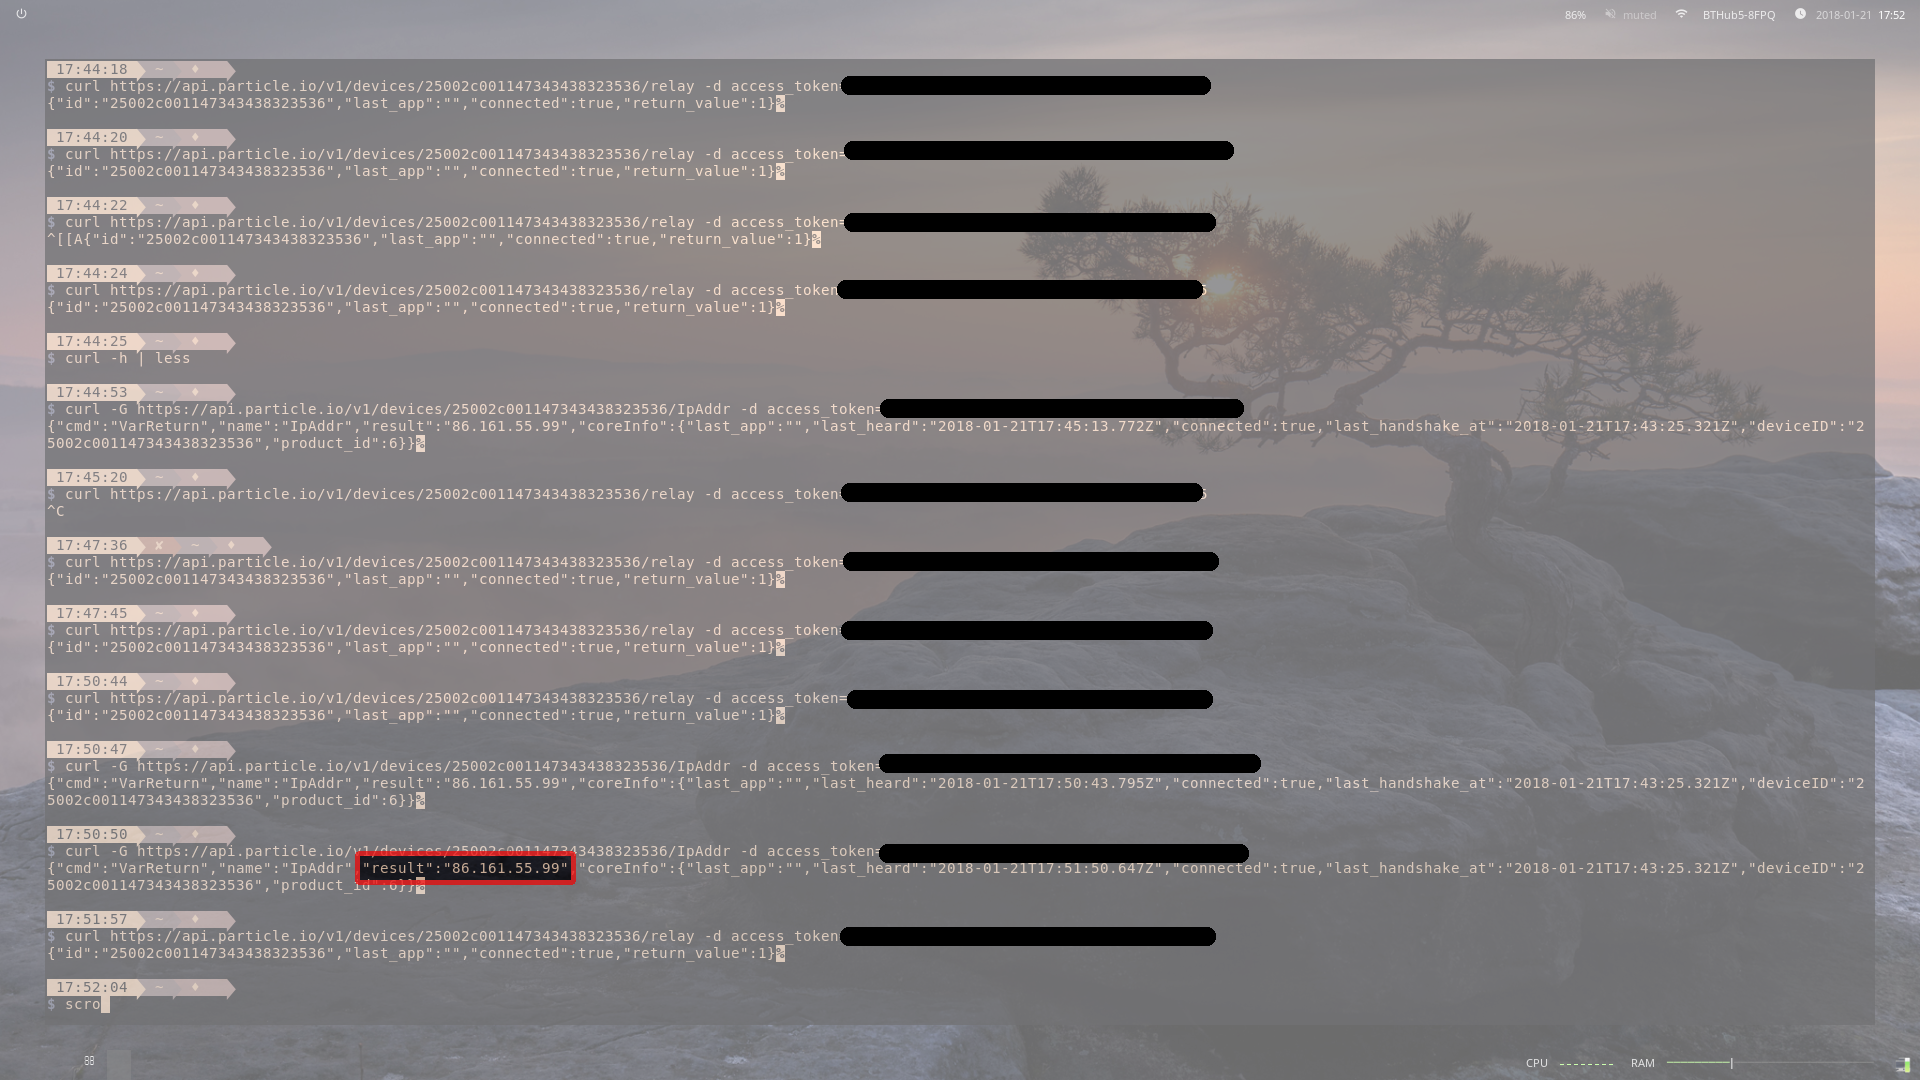
\includegraphics[width=\paperwidth-3cm]{pictures/IpTest.png}};
    \caption{Ip test} \label{fig:ipTest}
    The ip address is shown in the red box and I have blacked out the access tokens for the request
    for obvious reasons.
\end{figure}

\subsection{The client interface}
This section will talk about how I plan to implement a client that can trigger the boards functions
remotely. Since this is the design section as oppose to the build I will only out line how I plan to
do this without actually coding it. The first and foremost thing that the interface requires is a
way to communicate with server. At the moment with the design of the board we can communicate with
POST and GET http requests meaning I need a way of performing those actions. Fortunatly python has
many libraries that allow you to perform such actions. One of the most popular and the one that I
will be using for the interface is the requests library\cite{pythonRequests}. You can send get
requests using the "requests.get(<url>)" method where "<url>" is the url that you want to send the
request to. We will set this url to the one of the particle api.

To then connect to the server and communicate with it I can use the "pxssh" library and use that to
create a proper shell session between the server and the interface. I will go into details about
how I will program this in the interface section of the build section.


\section{Build}
In this section I will describe the process of me building this project

\subsection{Client Interface}
Originally I thought the best approach to connect to the server through ssh was to use a third party library
but after some experimentation I discovered that using the "os.open" command instead was significantly
easier and was much more effective at the job. This does mean however that it will only run on unix systems
with ssh install but considering in my previous solution you would need to install a library it is not
much of a disadvantage. Fortunatly that was the only change that was needed from my original plan. I have
listed the code below and will describe everthing it does.

\begin{mdlisting}
        \lstinputlisting[language=python, caption=\mylstcaption, label=lst:c1]{../src/interface.py}
\end{mdlisting}

The first thing to consider is the options dictionary which is use to store all of
the operations that the user can perform. The options that are displayed to the user
are store as a key in the dictionary while the values are then used to store the
relevant procedure. Other key variables in this are "ip\_address", "access\_token"
and "url". The ip\_adress variable is used to store the public ip address of the server
and is updated through the getIp() procedure. The "access\_token" variable stores
the access token needed by the api to give it correct permissions to perform actions.
Finally "url" is used to store the url of all of the api requests that we are going to
perform.

\subsection{The Hardware}
The first and most important thing for me to do was to connect the particle photon to the
server so that it could be remotely controlled. This was easy to do but did require some
solder which I will explain here.

\subsubsection{Soldering}
Soldering is the process of joining wires and electrical components together. It is done
by heating a soft alloy called solder and heating it up till it melts. While in this molten
state you can attach the components needed. In order to heat the solder you need a piece of
equitment called a soldering iron. It is good practive to first clean the soldering iron
before you turn it on by scratching off the outmost layer with sand paper. Once this is
done you can tin the solder iron which is where you apply solder the iron while it is still
heating it up to provide a protective layer. Once this setup is done you can finally begin to
solder. When soldering you should first heat the components with the soldering iron and then
feed the solder into the join.


\subsubsection{Connecting the photon to the server}
The first thing that I did was to remove the switch that was attached to the server. This was easily
done with a pair of wire cutters. Once this was done I use some wire strippers to get rid of the
insulation on the wires so that I could begin soldering. I then twisted the copper wires together
so there were no individual strands so that I could then tin the coper bit with solder. I did this
by first taping the wire down so it couldn't move and then heat the copper part with my solder iron
and placed solder along it. I did this to both server wires along with the wires that would connect
the relay sheild and the server. The reason why I tinned theses wires is because when it comes
to connecting them it is significantly easier when both wires already have solder on them. With these
tinned I connected the wires with additional solder to the outgoing wires and wraped them in electrical tape.
I did this to stop the wires from turning on the server if they touch one another. Finally I connected the
outgoing wires to the relay.


\begin{figure}[H]
    \begin{center}
        \begin{tabular} {ccc}
            \subfloat[Pictue of soldering iron]{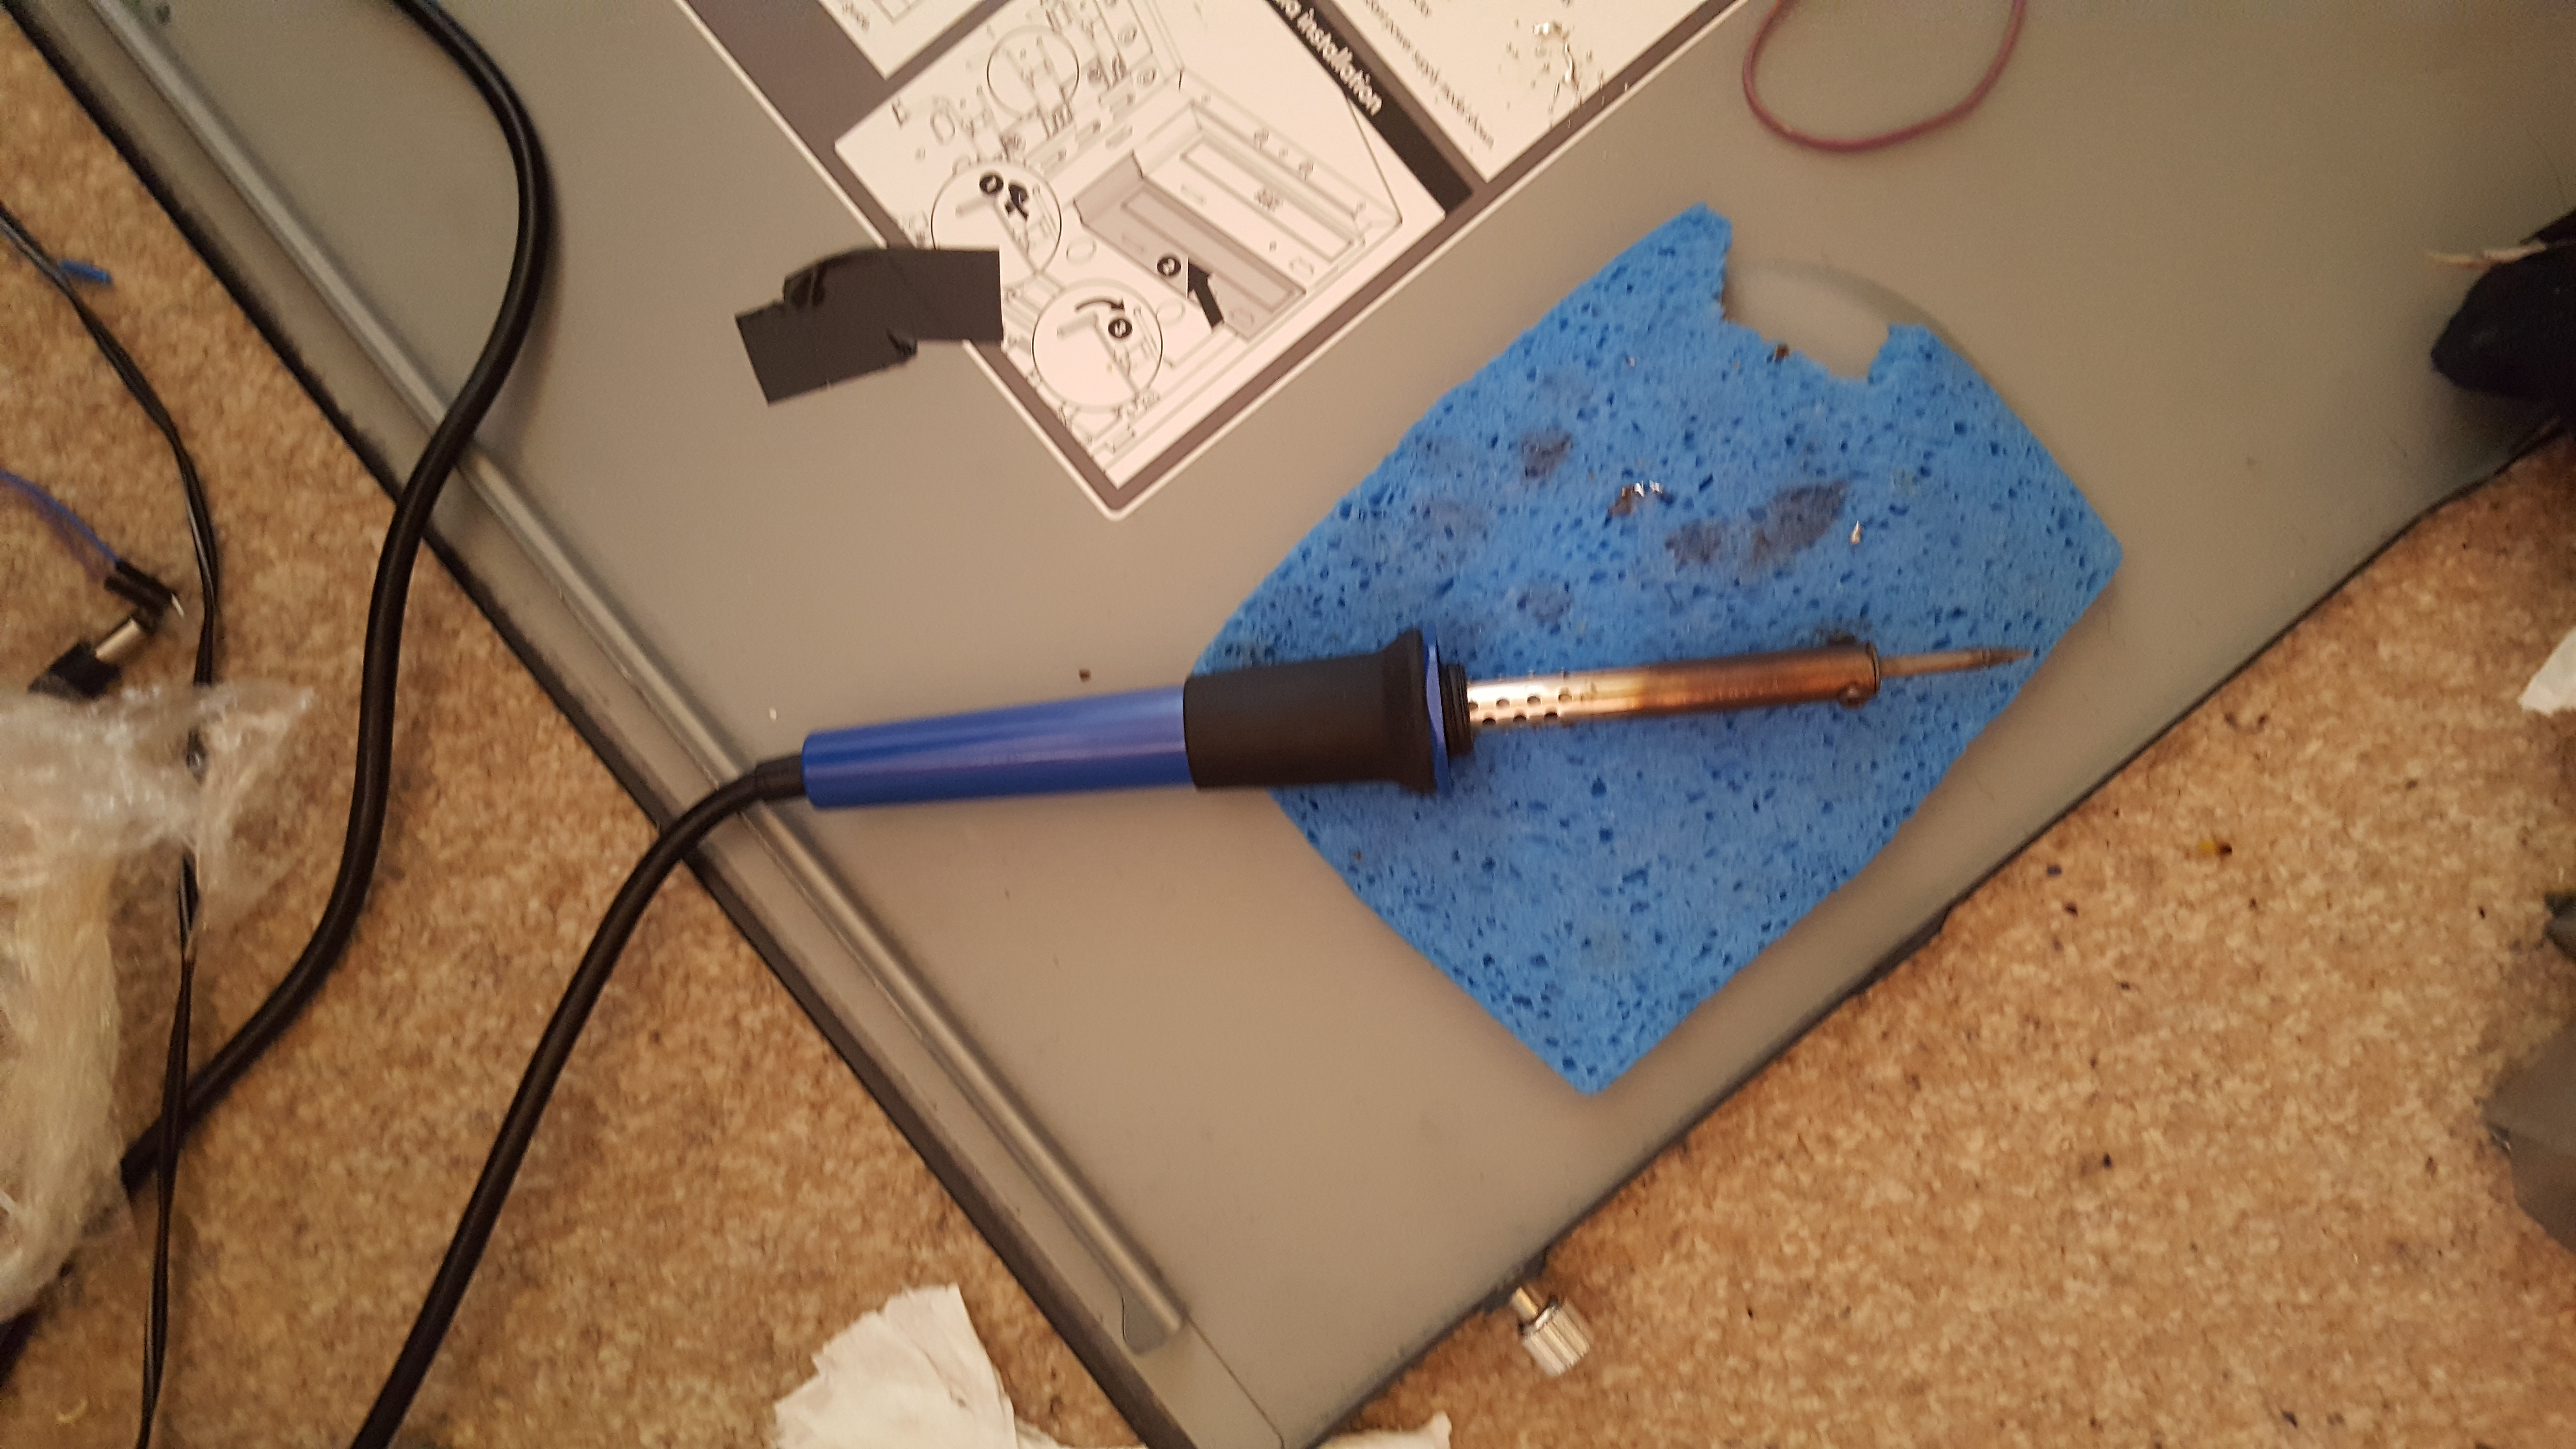
\includegraphics[width = 2in]{pictures/camera/solderIron.jpg}} &
            \subfloat[Picure of server wires before soldering]{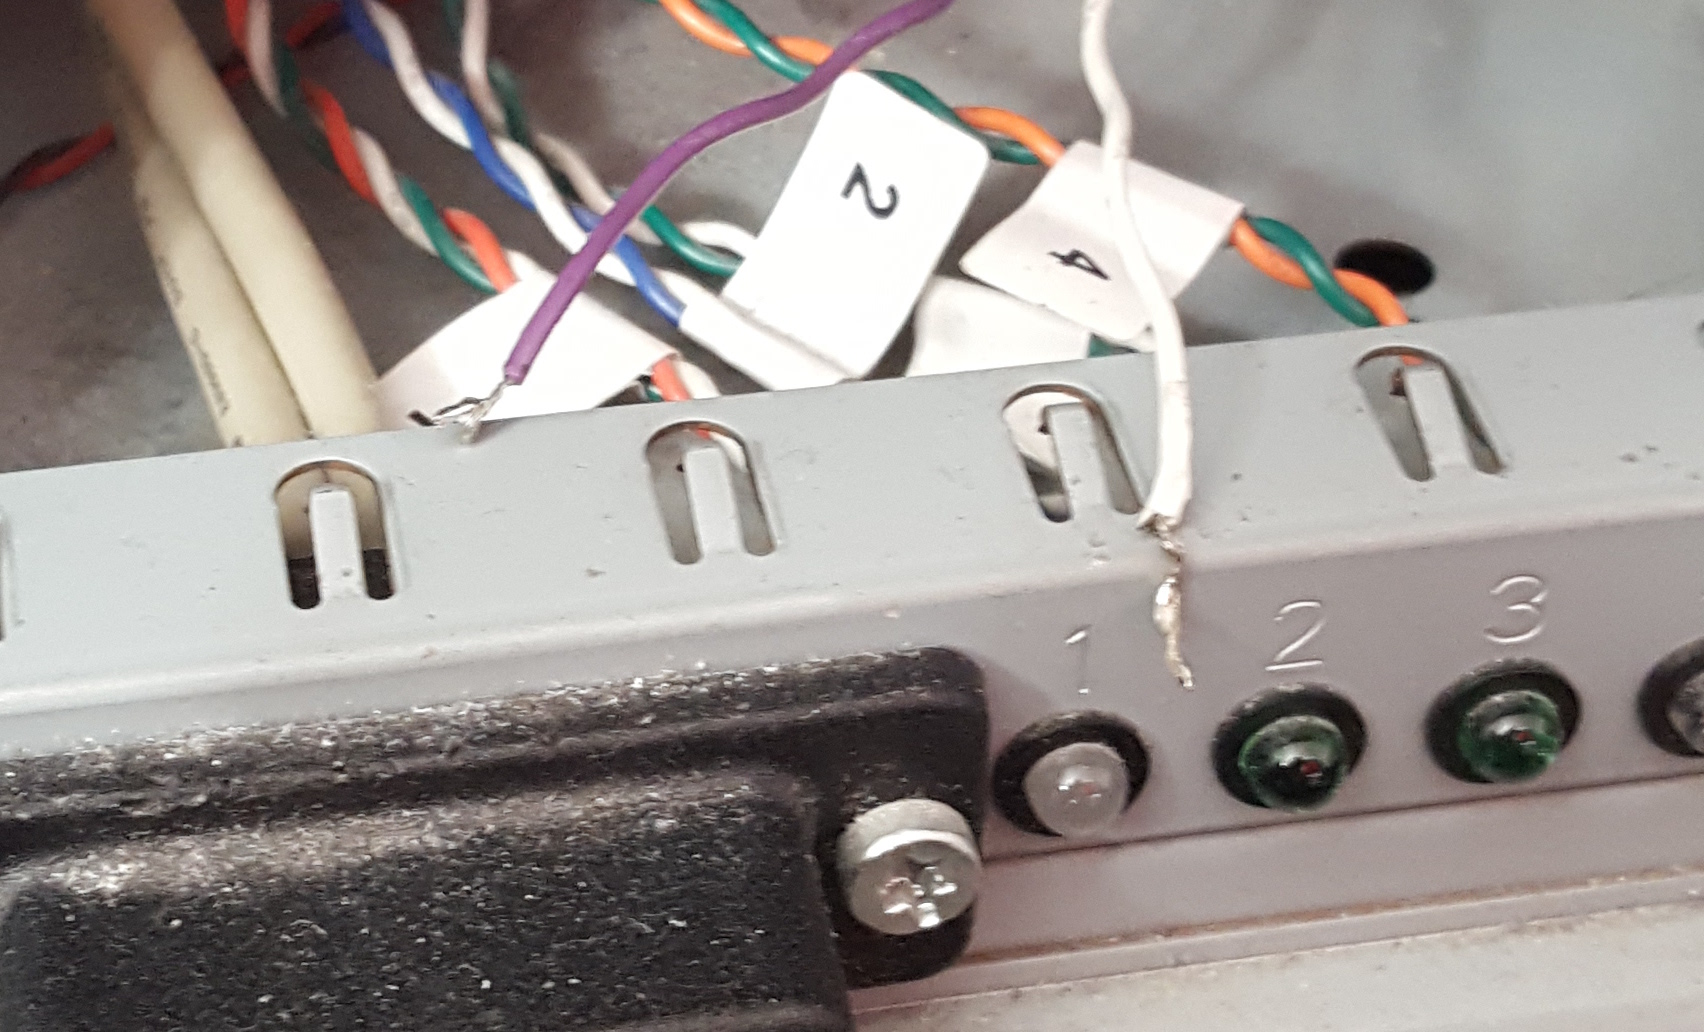
\includegraphics[width = 2in]{pictures/camera/unSolderServerWires.jpg}} &
            \subfloat[Picture of taped down wire]{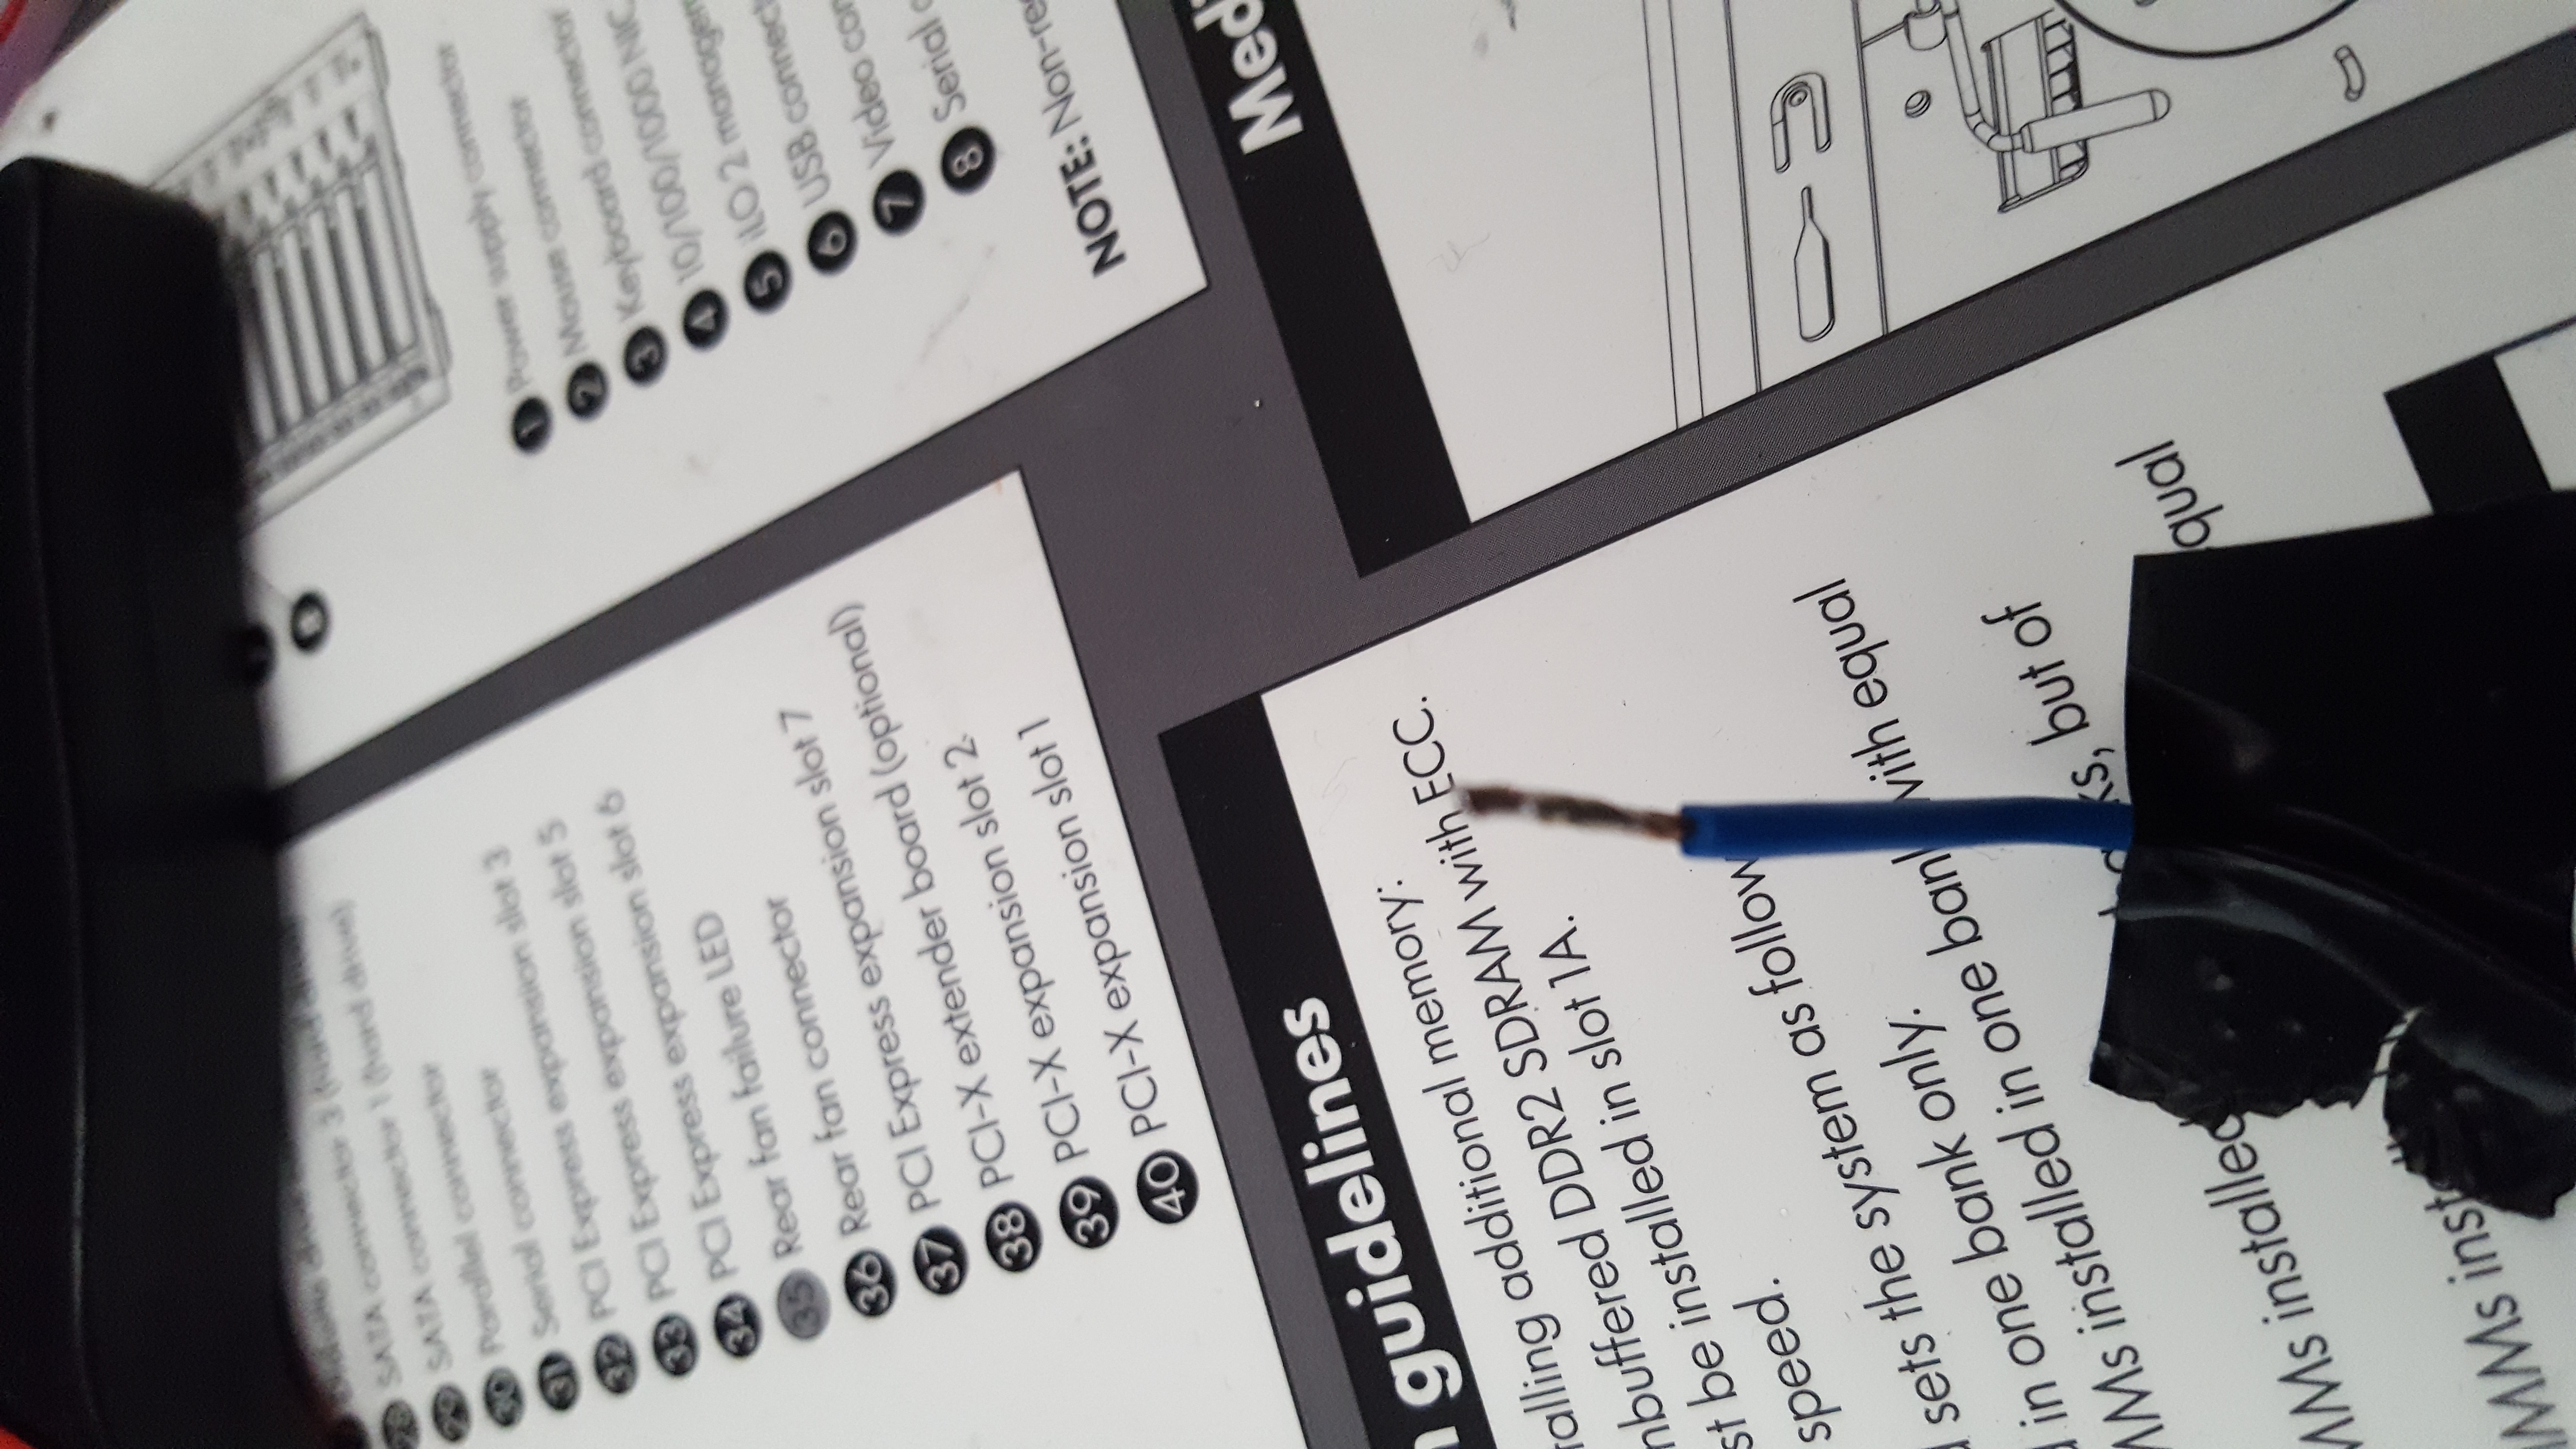
\includegraphics[width = 2in]{pictures/camera/tapedServerWire.jpg}} \\

            \subfloat[Soldered Wires]{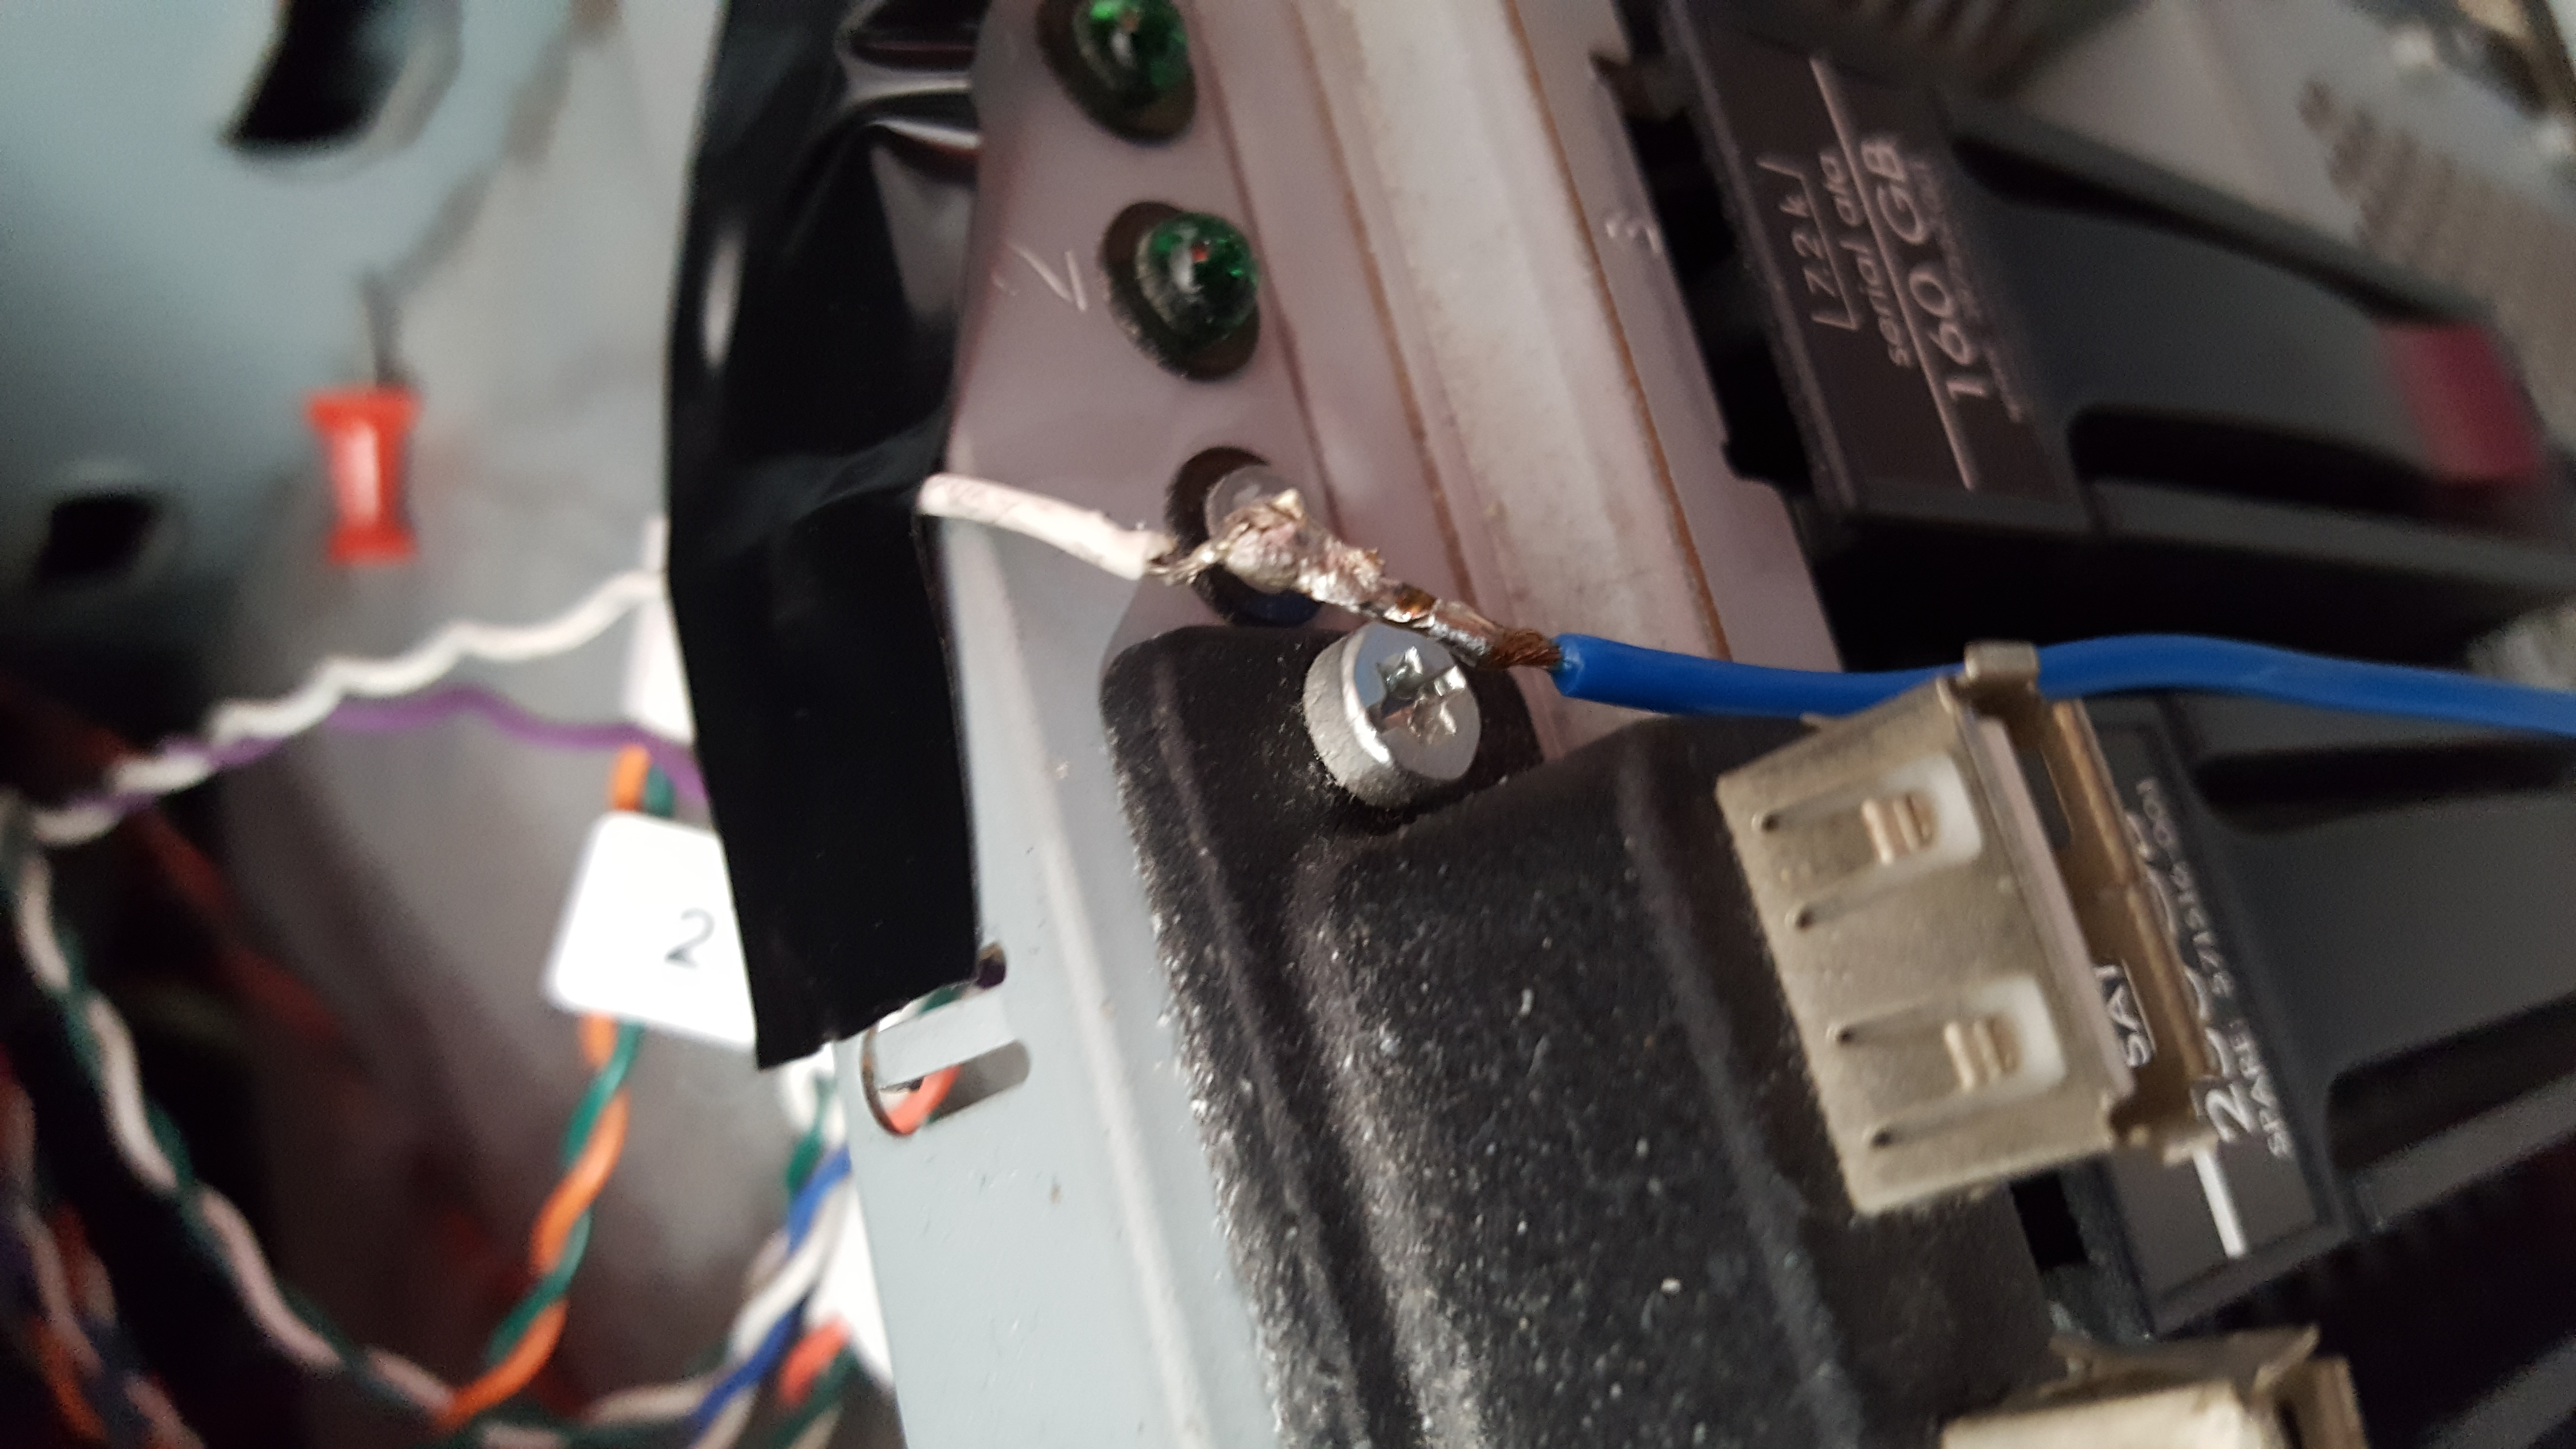
\includegraphics[width = 2in]{pictures/camera/solderServerWiresNewest.jpg}} &
            \subfloat[Wires insulated after soldering]{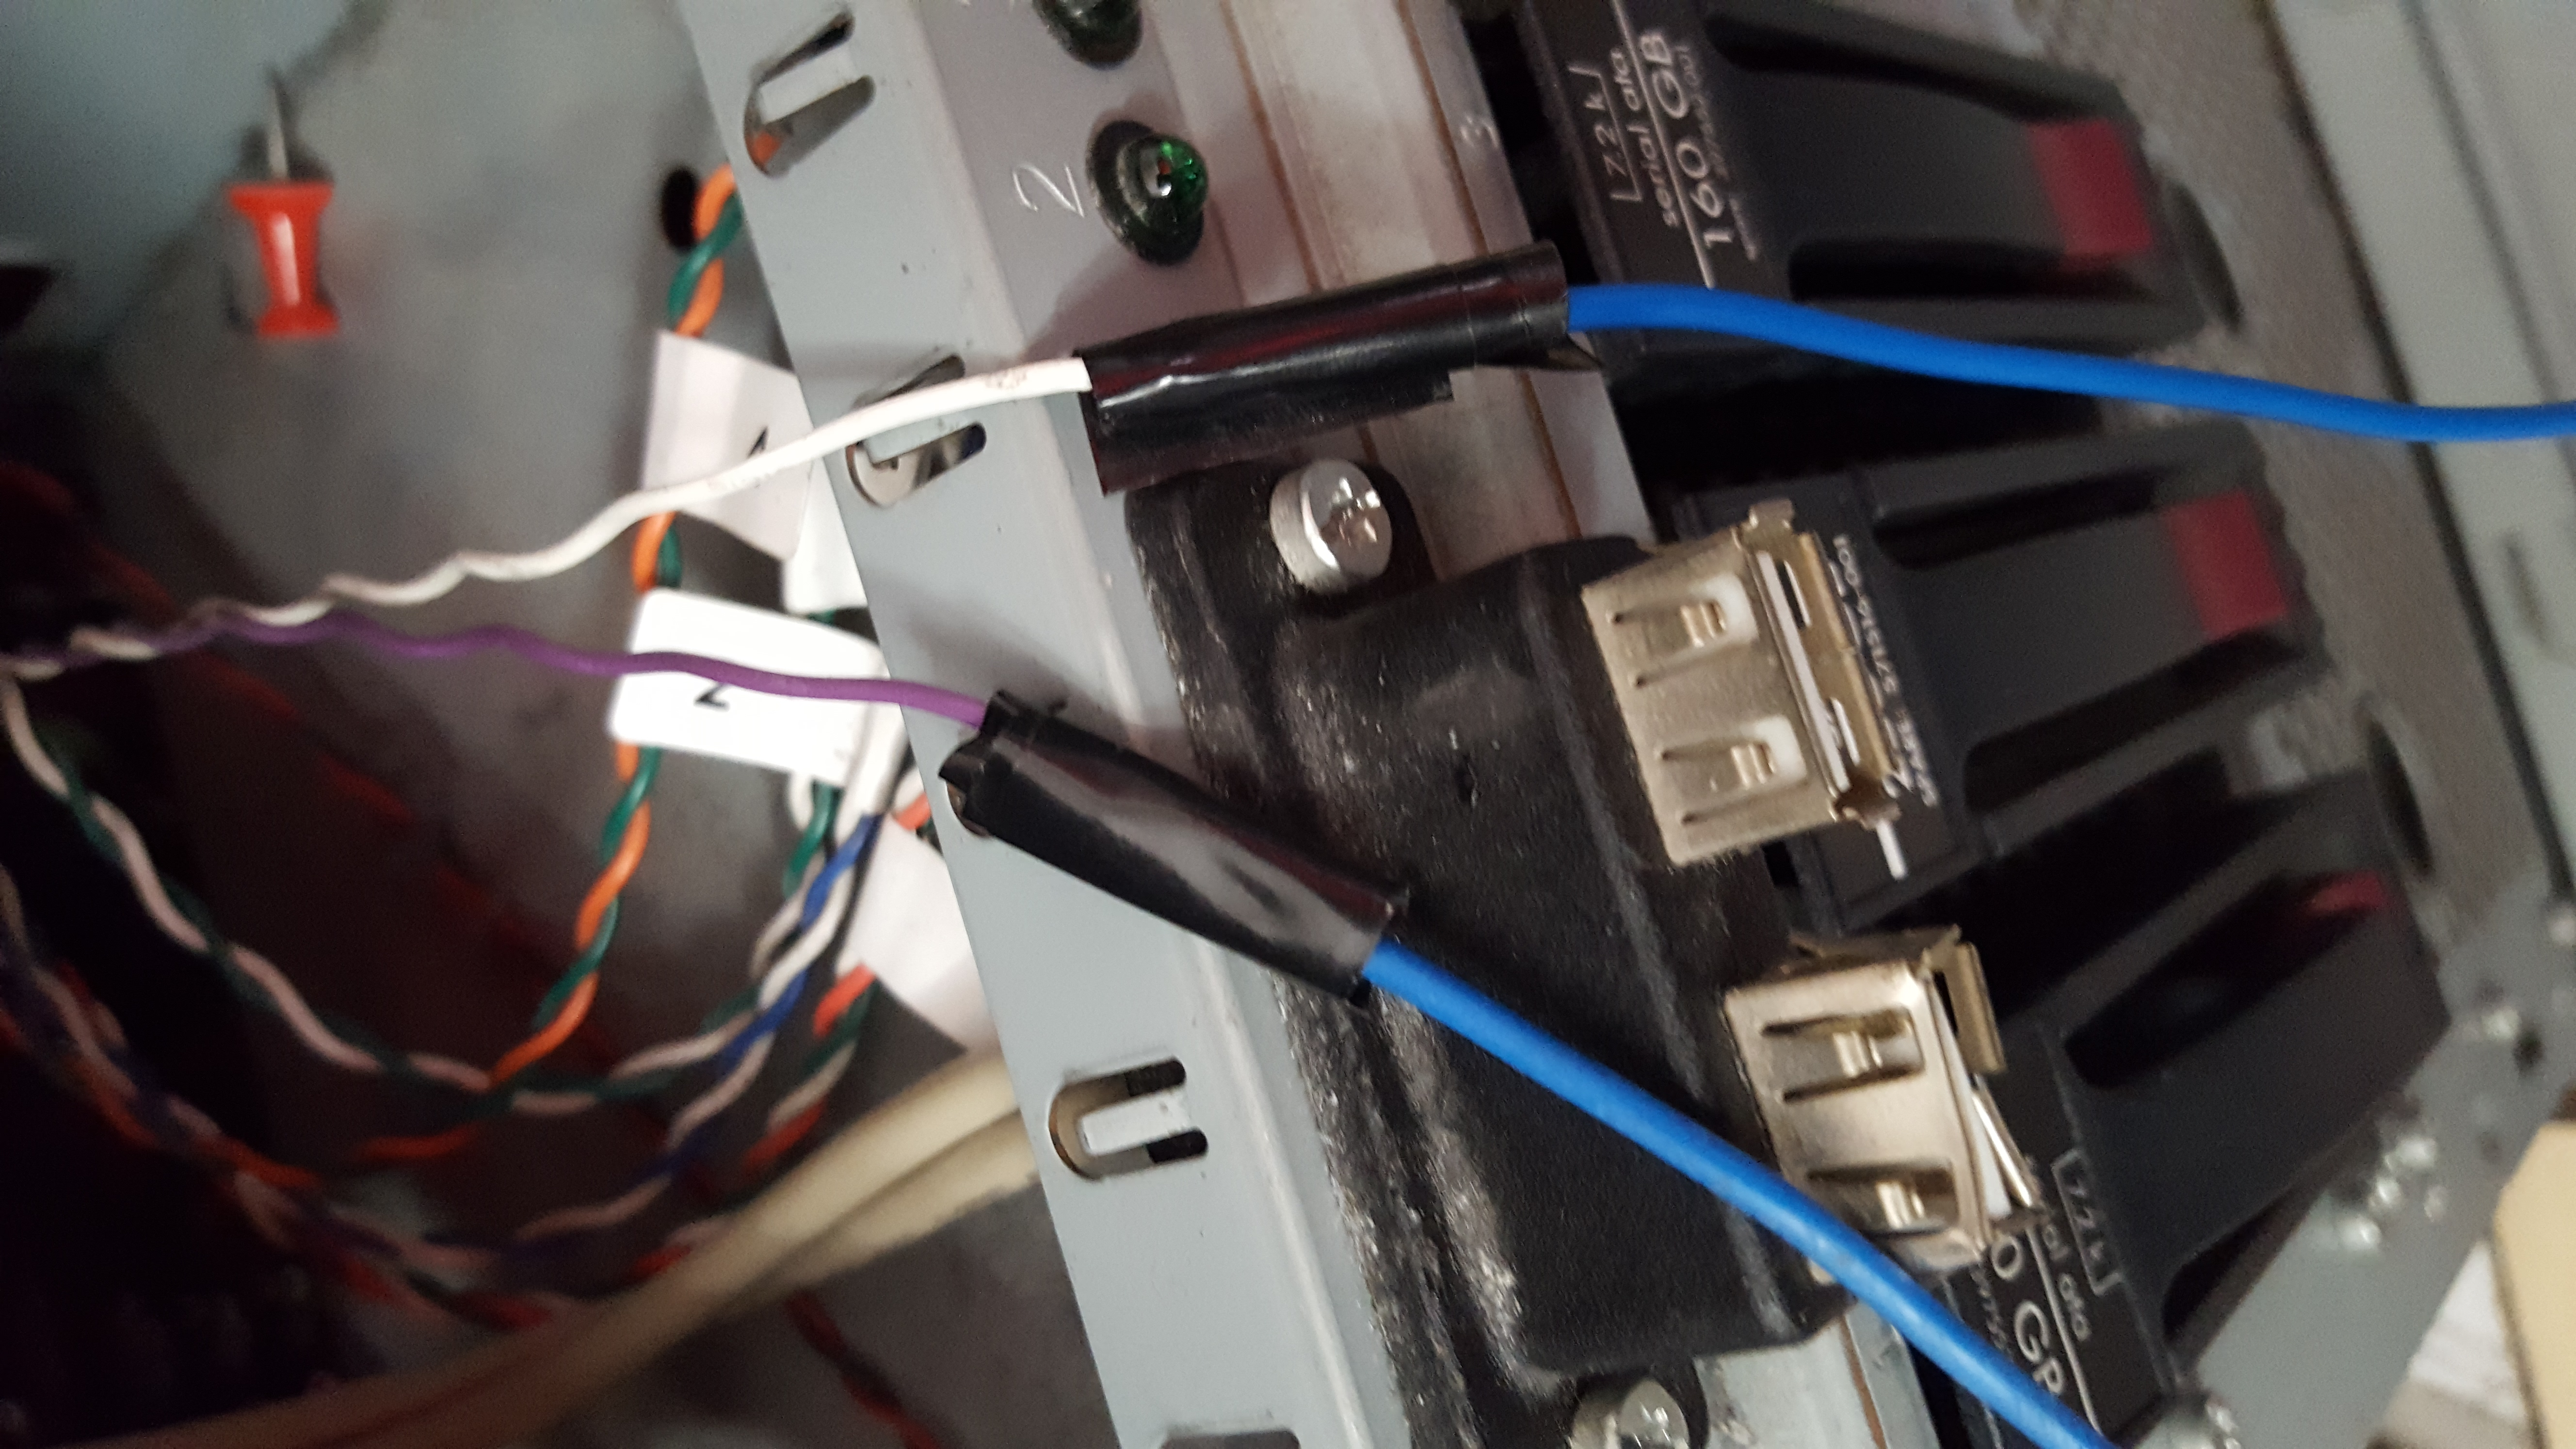
\includegraphics[width = 2in]{pictures/camera/serverWiresConnectedAndInuslated.jpg}} &
            \subfloat[Outgoing wires connect to relay]{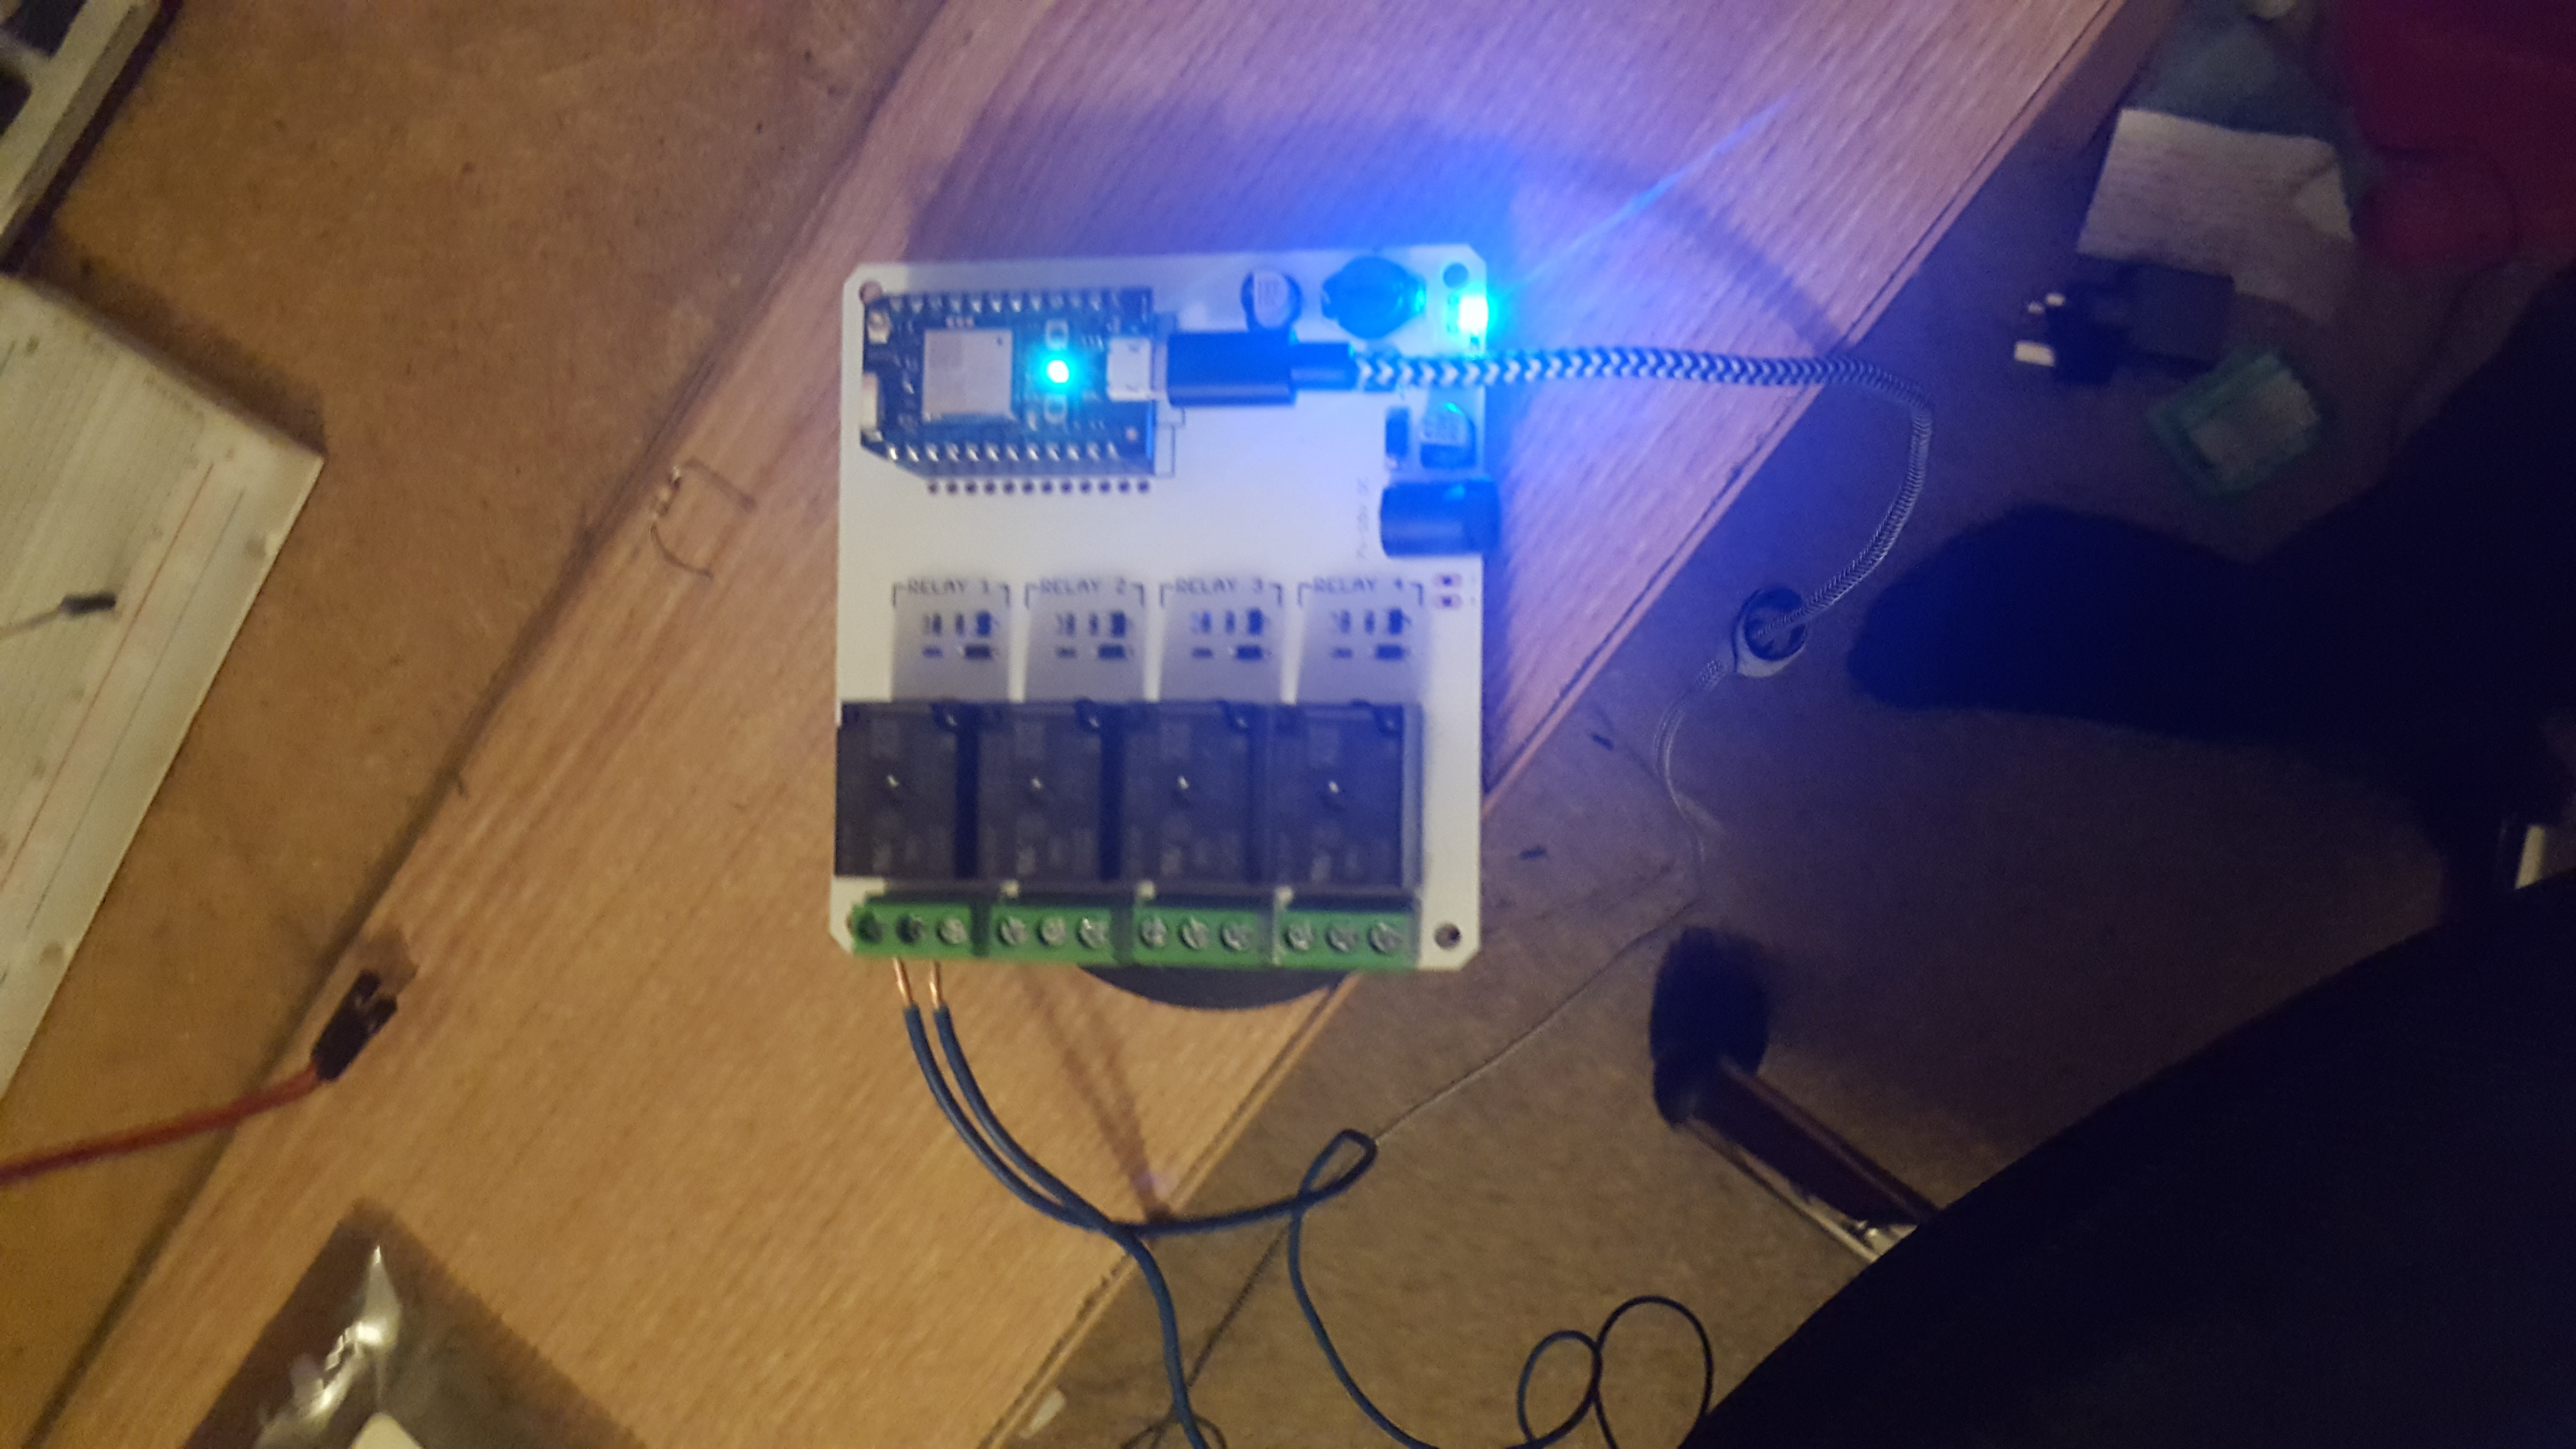
\includegraphics[width = 2in]{pictures/camera/outGoingWiresToRelay.jpg}} \\
        \end{tabular}
    \end{center}
    \caption{Photos of build} \label{fig:photonServerPicsBuild}
\end{figure}


\subsubsection{Connect the server power cord to the photon}
The next thing that needed to be done was to the mains power supply to the server to the photon
so that it can regulate the power supply. In order to do this I needed to understand what cables
run in the mains power supply and how I can manipulate these wires to control the server. The mains
power supply consists of three wires: the neutral wire which is blue; the live wire which is brown
and the earth wire which has green and yellow strips for clouring. I was not sure whether the
server uses earth or not so I thought it would be best not to attach the relay to the earth wire. Because
of this I chose the neutral wire as I was sure this would have the desired affect on the server.
The first thing for me to do was to strip away the outer insulation to revel the three wires. I did this
with a knife by first cutting circles around the wire at certain points and then making a straight
line incision between these two circles. I the cut the neutral wire and strip off the insulation on
both ends. After twisting the coper innerards I attached it to the relay. I did however attached it
differently to the relay as I wanted this to be in an "normally close" state. This meant do both
the middle pin and the far right pin.

Once this was done it was time to add the manual override switch. This was easy to do as I could connect
the switch in the live wire of the mains power supply to the server. The first thing I had to do was
to cut the wire and strip the insulation off. After this was done I twisted the copper core together and
threaded it through the hole of the switch. I then soldered this in place and wrapped each end with
electrical tape.


\begin{figure}[H]
    \begin{center}
        \begin{tabular} {ccc}
            \subfloat[Pictue showing the three wires]{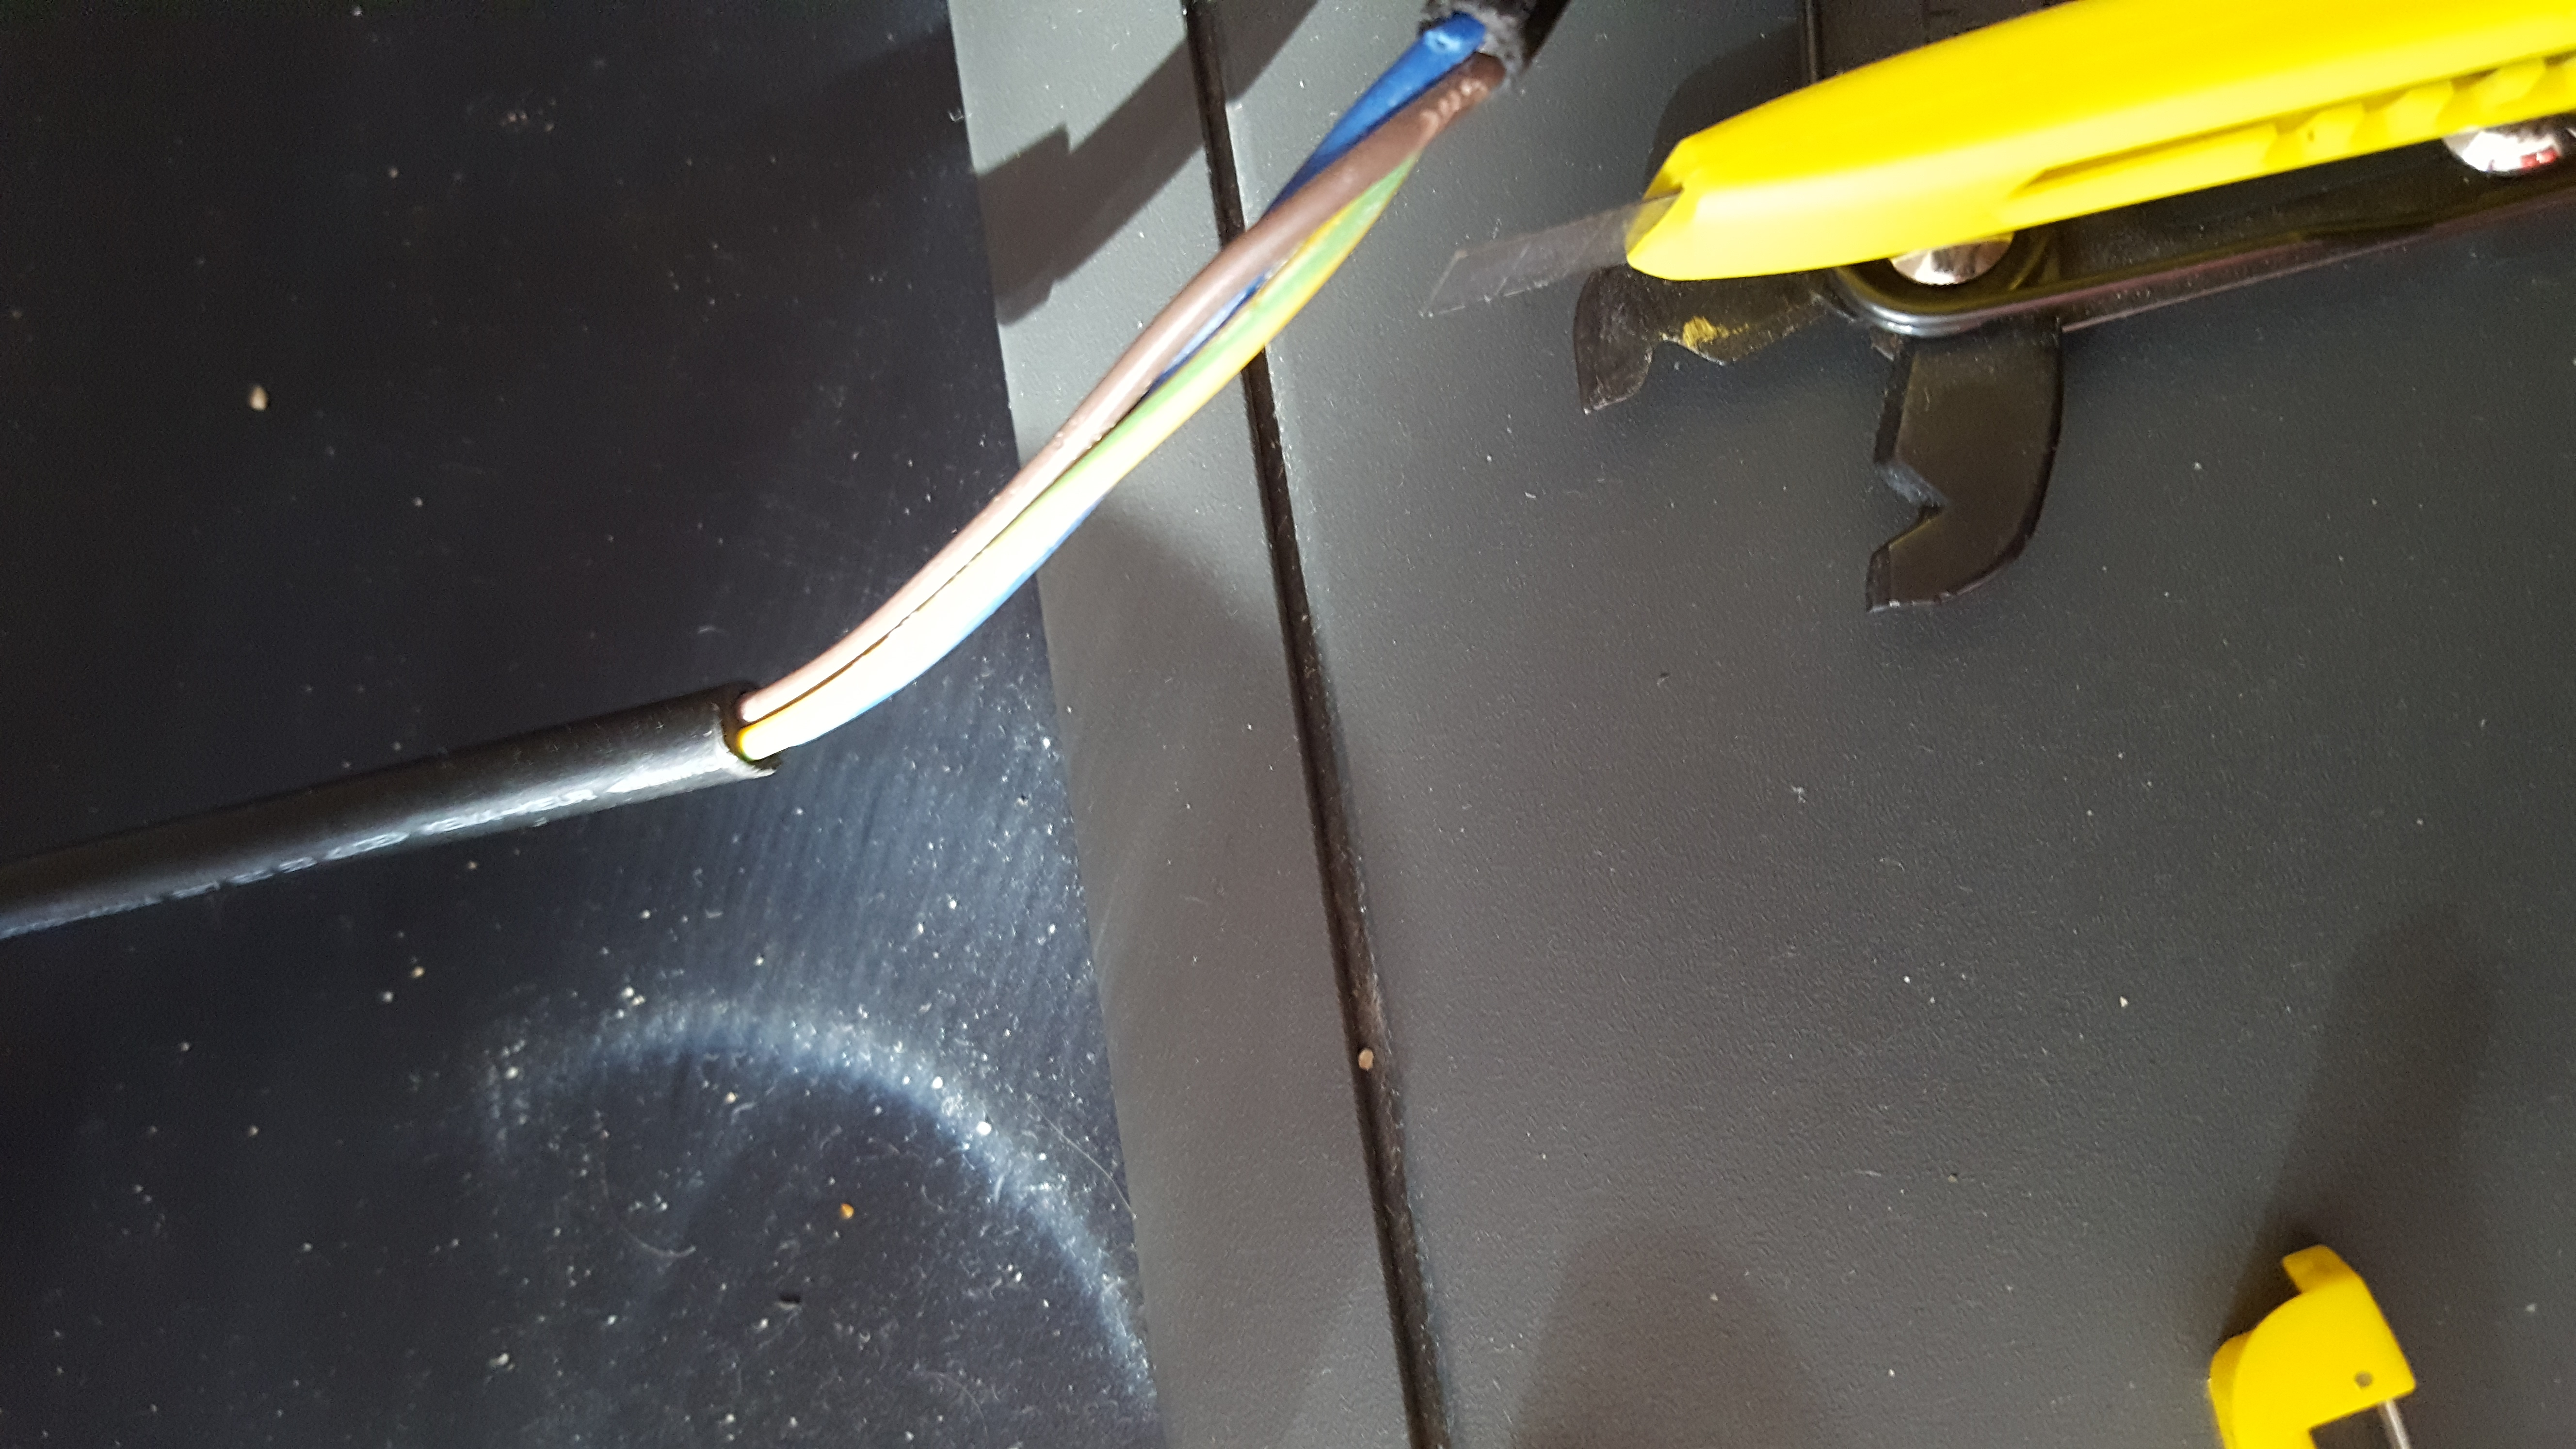
\includegraphics[width = 2in]{pictures/camera/removeOuterInsulationMainsWire.jpg}} &
            \subfloat[Pictue showing all the wires connected to the relays]{\includegraphics[width = 2in]{pictures/camera/variousWiresConnectedToRelay.jpg}} & \\
            \subfloat[Pictue showing wires threaded through switch]{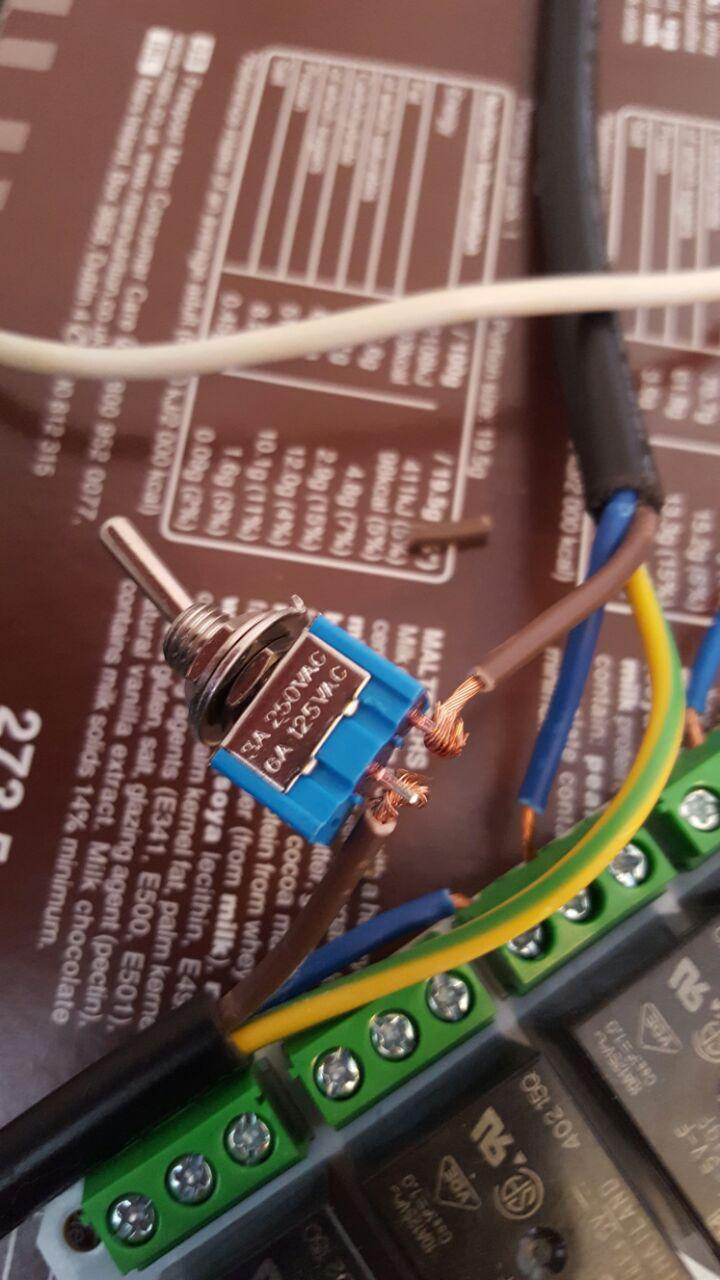
\includegraphics[width = 2in]{pictures/camera/theadedSwitch.jpg}} &

            \subfloat[Pictue showing the wires soldered to switch]{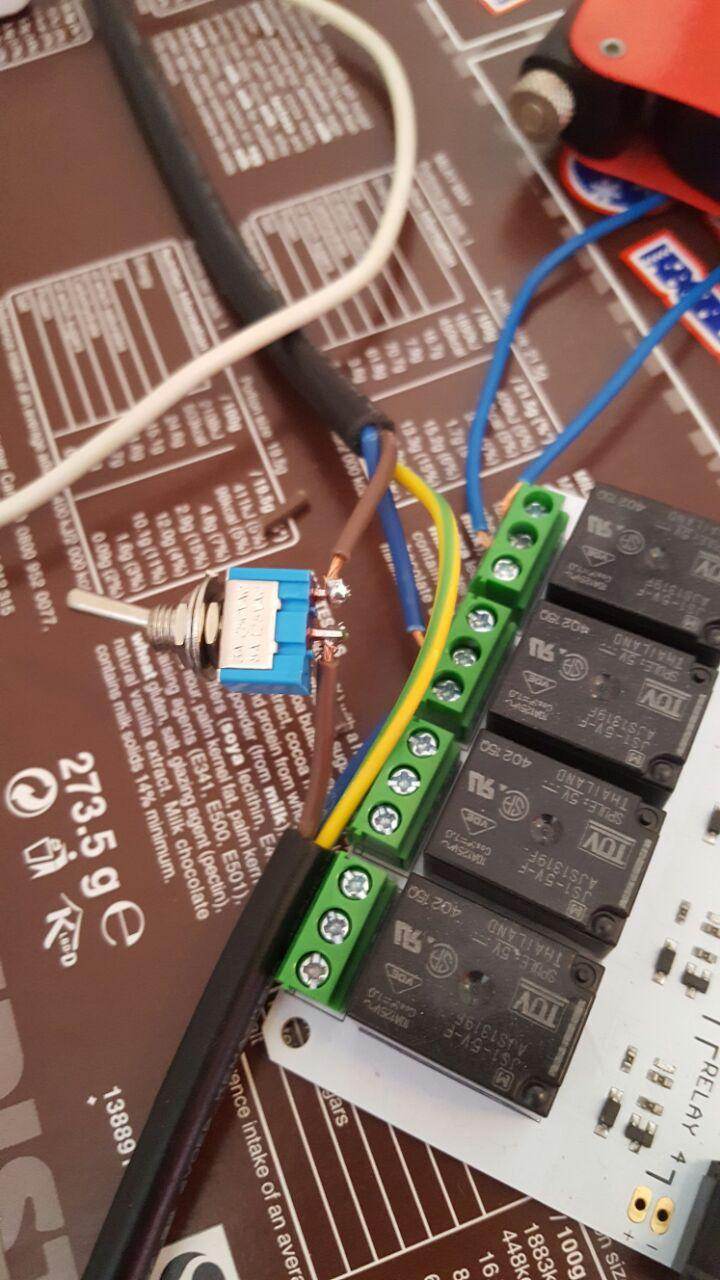
\includegraphics[width = 2in]{pictures/camera/solderSwitch.jpg}} &
            \subfloat[Pictue showing the switch insulated]{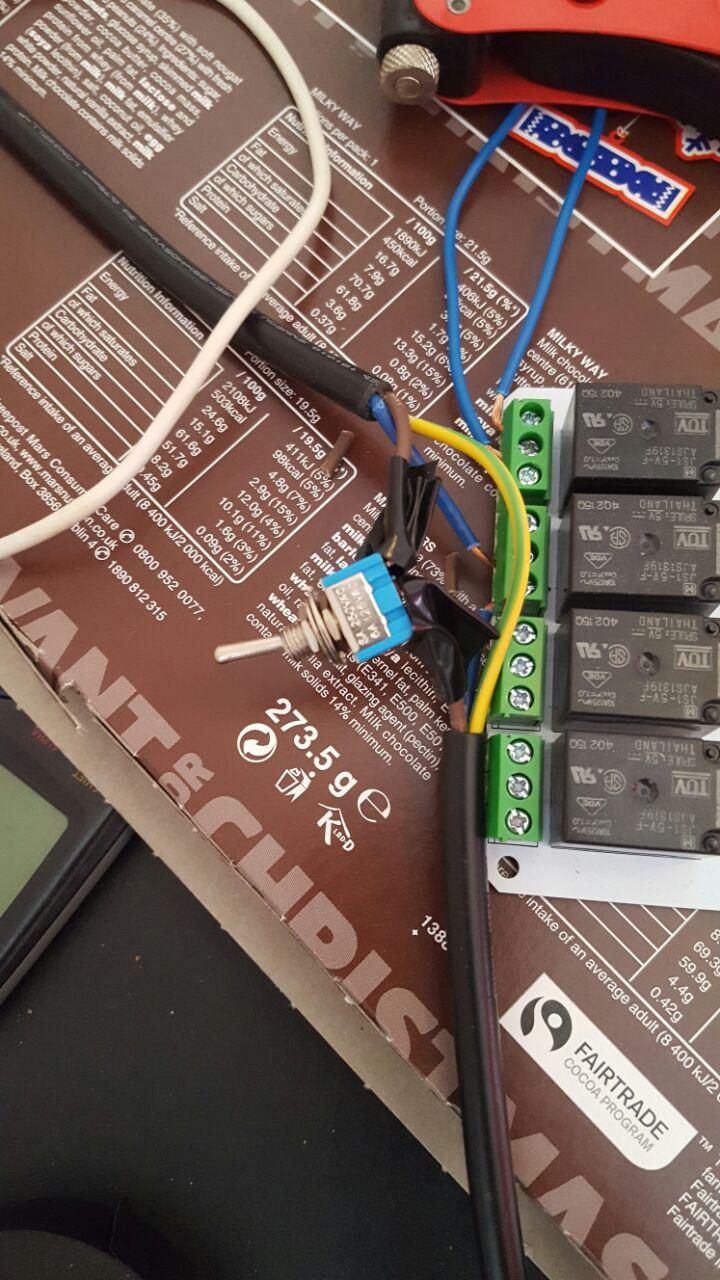
\includegraphics[width = 2in]{pictures/camera/insulatedSwitch.jpg}} \\
        \end{tabular}
    \end{center}
    \caption{Photos of build} \label{fig:photonServerPicsBuild}
\end{figure}

\subsubsection{Connect the server usb power to the photon}
The final thing to do in the build is to connect a relay up to the server usb and the power supply of
the particle photon so that when the server turns on the photon is turned off. The start of this process
is similar to the previous section as I need to remove the outer insulation of cable powering the photon
and then select the correct wire. In this case however there are four wires. Two for data, two for power.
I'm only interested in the power ones which are labeled red and black. It doesn't matter which of these
wires I choose but I decided to use the red one. I then need to take the power from the usb outlet which
is simple to do from a old usb cable. All that is needed is to cut the wire and extract the red and black
wires to power the relay. Once this is done I just need to connect the appropitate wires to the correct
places. The power to the photon board should go across normally close while the power from the server
usb should go across the coil. I then solder these wires in place and coverer the ends in insulation
tape. Interestingly the usb wire I connected to the server did not have same colours as the wires
in the other usb cable. This is likely due to the one connected to the server having a ground
wire. To figure out the power cables for this wire I used a multi metre to measure the voltage across
the two of the wires until it read out 5 volts. When it read out this 5 volt value I knew those two
wires are the one responsible for power. I also had to apply lots of electrical tape as I needed to
ensure that the pins were properly insulated.


\begin{figure}[H]
    \begin{center}
        \begin{tabular} {ccc}
            \subfloat[Removed outer insulation on usb]{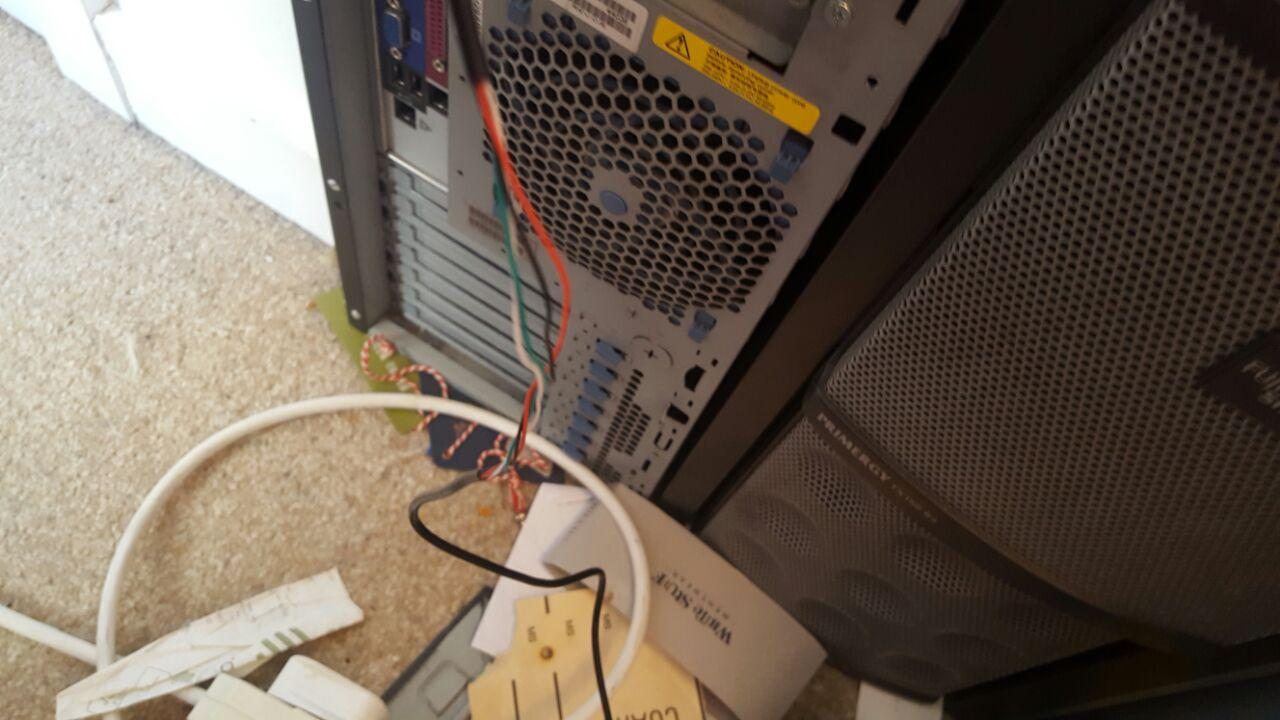
\includegraphics[width = 2in]{pictures/camera/phtonPowerOuterInsulationRm.jpg}} &
            \subfloat[Tined photon power wires twisted around pins on relay]{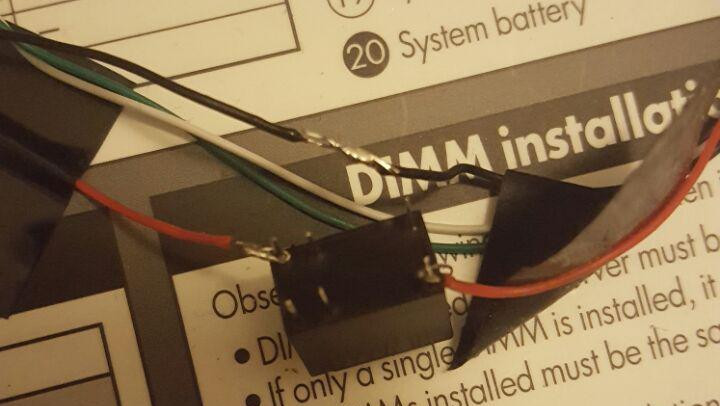
\includegraphics[width = 2in]{pictures/camera/hookedPreSolderExtRelay.jpg}} &
            \subfloat[Photon power wires soldered to relay]{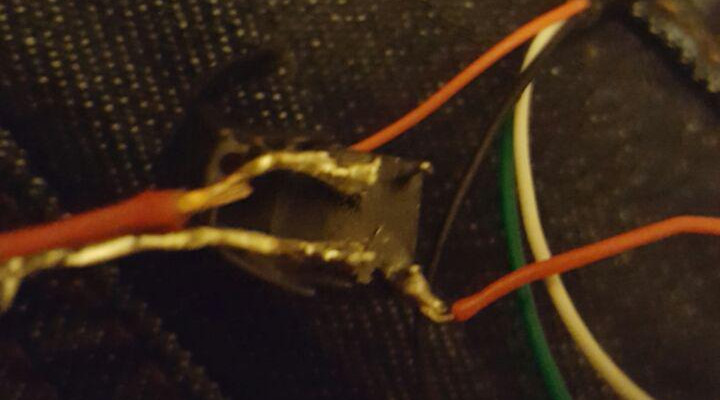
\includegraphics[width = 2in]{pictures/camera/solderedExtRelay.jpg}} \\
            \subfloat[Finding correct wires with multimetre]{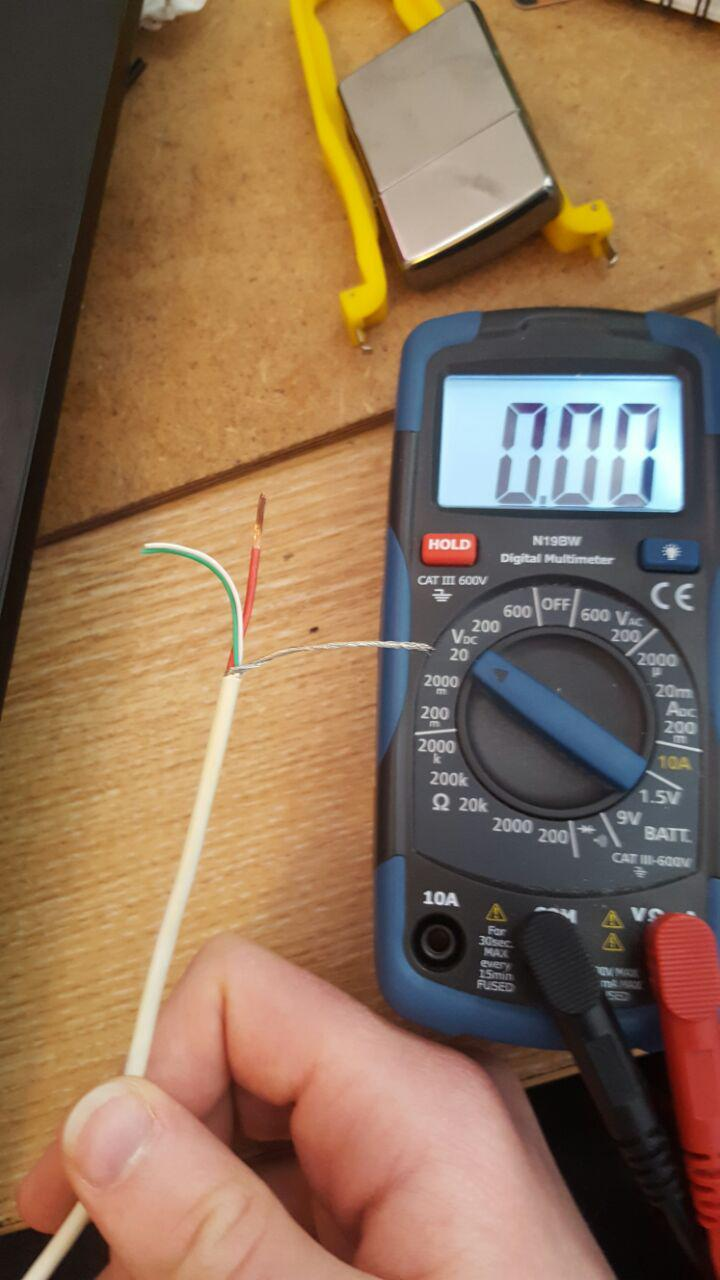
\includegraphics[width = 2in]{pictures/camera/multiMetre.jpg}} &
            \subfloat[Insulated solder bit with electrical tape]{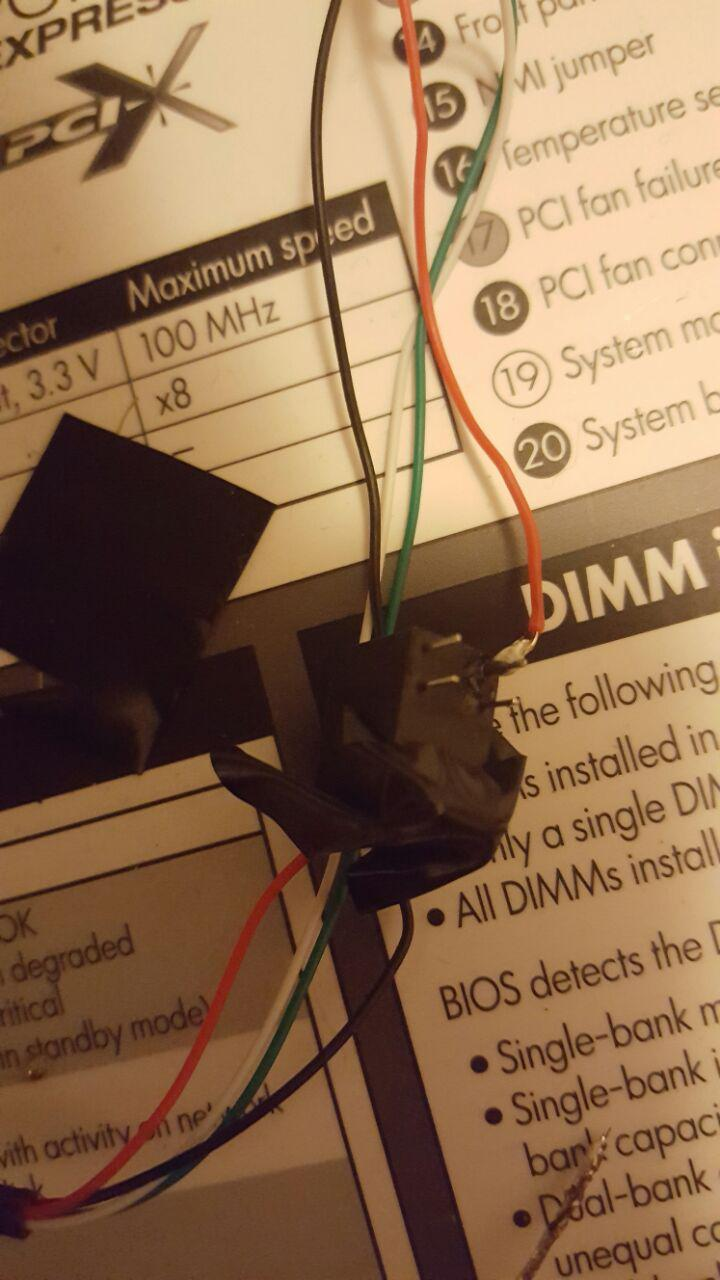
\includegraphics[width = 2in]{pictures/camera/halfInsulatedExtRelay.jpg}} &
            \subfloat[Soldered and Insulated the rest of the wires]{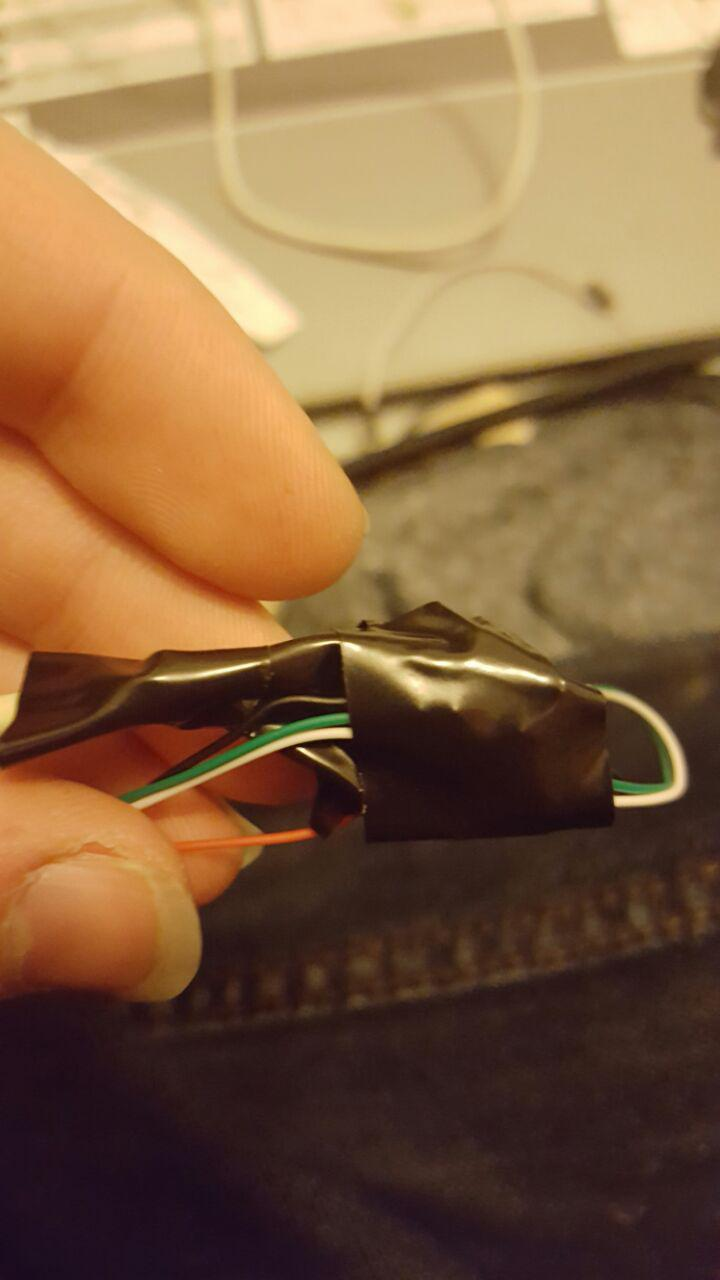
\includegraphics[width = 2in]{pictures/camera/fullyInsulatedExtRelay.jpg}} \\
        \end{tabular}
    \end{center}
    \caption{Photos of build} \label{fig:photonServerPicsBuild}
\end{figure}

\subsection{Code for the photon}
There are some minor alterations that need to be made for the photon board. This mainly to turn on relay 2 at the start.


\begin{figure}[H]
    \begin{lstlisting}
    int RELAY1 = D0;
    int RELAY2 = D1;
    char ip[15];

    void setup()
    {
       //Initilize the relay control pins as output
       pinMode(RELAY1, OUTPUT);
       pinMode(RELAY2, OUTPUT);
       // Initialize all relays to an OFF state
       digitalWrite(RELAY2, HIGH);
       digitalWrite(RELAY1, LOW);

       //register the Particle function
       Particle.function("relay", relayControl);\
       Particle.variable("IpAddr", ip);
       Particle.subscribe("particle/device/ip" , handler);
       Particle.publish("particle/device/ip");

    }

    void handler(const char *topic, const char *data)
    {
        strcpy(ip, data);
    }

    // command format r1,HIGH
    int relayControl(String command)
    {
        digitalWrite(RELAY2, 0);
        delay(1000);
        digitalWrite(RELAY1, 1);
        delay(500);
        digitalWrite(RELAY1, 0);

        return 1;
    }
    \end{lstlisting}
    \caption{Final code for controller} \label{fig:interfaceCode}
    \vspace{0.5cm}
\end{figure}


\section{Evaluation}

Overall i'm happy with the result of the project as it meets all of the goals that I set out at
the start. I think the power consumption of the device is at an absoulute minimal this has however
come at a cost which you can see below in figure \ref{fig:costTable}.

\begin{figure}[H]
    \begin{center}
        \begin{tabular} {| c | c |}
            \hline
            \textbf{Item}                 &      \textbf{Cost}      \\ \hline
            Particle photon dev Board     &         £17.00          \\ \hline
            Relay sheild                  &         £25.00          \\ \hline
            Switch                        &         £0.00           \\ \hline
            External relay x5             &         £6.65           \\ \hline
            Wire                          &         £0.00           \\ \hline
            Micro usb wires x2            &         £0.00           \\ \hline
            \multicolumn{2}{ | c |}{\textbf{Total: £48.65}}         \\ \hline
        \end{tabular}
    \end{center}
    \caption{Cost table} \label{fig:costTable}
    \vspace{0.5cm}
    The items with the cost of £0.00 are items that I already had before the start of this project.
\end{figure}

The total price is not below my maximum budget but is definetly higher than I would like it to
be. The price could have been significantly lower if I used some of the spare external relays
instead of buying the relay sheild. That being said doing this would be hard to acheieve within
the time restraints.

Time became an issue during this project, I think this mainly because I spent too long on the research
and should have use that time on the design section as I had a lot of other matters to attend to during
that period. The build and evaluation took shorter amount of time than original outlined.

Although the final build does everything that I set it out to do I think it can be extended by adding
some of the interace functionality to a discord bot. This would mean I would be able to interact with
the server on any platform and allow others to easily communicate with it as well. I also think it would
be good to automatically disable the turn on features between certain times as when the server comes on
it can be noisy and prevent people from sleeping.

\section{Information}

\begin{thebibliography}{56}

\bibitem{raspberryPi}
    \begin{itemize}
        \item Information for the raspberry pi was gather at this website
        \begin{itemize}
            \item Article title: Maker Shed: Arduino | Raspberry Pi | 3D Printers | Microcontroller Kit
            \item Website title: Maker Shed
            \item URL          : \url{https://www.makershed.com/pages/raspberry-pi-comparison-chart}
        \end{itemize}
    \end{itemize}

\bibitem{beagleboard}
    \begin{itemize}
        \item Information for the specs was found on this website
        \begin{itemize}
            \item Article title: Selecting BeagleBoard Hardware | DigiKey
            \item Website title: Digikey.com
            \item URL          : \url{https://www.digikey.com/en/product-highlight/t/texas-instruments/beagleboard}
        \end{itemize}

        \item Information for the price of a begalbone kit
        \begin{itemize}
            \item Article title: BeagleBone Black Wireless Starter Kit
            \item Website title: Amazon.com
            \item URL: \url{https://www.amazon.com/BeagleBone-Black-Wireless-Starter-Kit/dp/B01NGTOX40/ref=sr_1_2?ie=UTF8&qid=1510164000&sr=8-2&keywords=beaglebone+wifi&dpID=51g7KiFRteL&preST=_SY300_QL70_&dpSrc=srch}
        \end{itemize}

        \item Information for the spec specifc to the BeagleBone black wireless
        \begin{itemize}
            \item Article title: BeagleBoard.org - black-wireless
            \item Website title: Beagleboard.org
            \item URL          : \url{https://beagleboard.org/black-wireless}
        \end{itemize}

        \item Information for the spec specifc to the BeagleBone black
        \begin{itemize}
            \item Article title: BeagleBoard.org - black
            \item Website title: BeagleBoard.org - black
            \item URL          : \url{https://beagleboard.org/black/}
        \end{itemize}

    \end{itemize}

\bibitem{ardino}
    \begin{itemize}
        \item Information and specs for the Ardino Uno was gathered at this website
        \begin{itemize}
            \item Author       : Arduino
            \item Article title: Arduino Uno | Make: DIY Projects and Ideas for Makers
            \item Website title: Make: DIY Projects and Ideas for Makers
            \item URL          : \url{https://makezine.com/product-review/arduino-uno/}
        \end{itemize}
    \end{itemize}

\bibitem{particlePhotonSpec}
    \begin{itemize}
        \item A product review for the particle photon
        \begin{itemize}
            \item Author       : Particle
            \item Article title: Particle Photon | Make: DIY Projects and Ideas for Makers
            \item Website title: Make: DIY Projects and Ideas for Makers
            \item URL          : \url{https://makezine.com/product-review/particle-photon/}
        \end{itemize}

        \item A datasheet for the particle photon
        \begin{itemize}
            \item Author       : Particle
            \item Article title: Particle
            \item Website title: Docs.particle.io
            \item URL          : \url{https://makezine.com/product-review/particle-photon/}
        \end{itemize}
    \end{itemize}

\bibitem{transistor}
    \begin{itemize}
        \item Information and specs for the Ardino Uno was gathered at this website
        \begin{itemize}
            \item Author       : SparkFun Kit
            \item Article title: Transistors - learn.sparkfun.com
            \item Website title: Learn.sparkfun.com
            \item URL          : \url{https://learn.sparkfun.com/tutorials/transistors}
        \end{itemize}
    \end{itemize}

\bibitem{relaySheild}
    \begin{itemize}
        \item Information regarding the particle photon relay sheild
        \begin{itemize}
            \item Author       : Particle
            \item Article title: Particle
            \item Website title: Docs.particle.io
            \item URL          : \url{https://docs.particle.io/reference/firmware/photon/#get-public-ip}
        \end{itemize}
    \end{itemize}

\bibitem{publicIPDocs}
    \begin{itemize}
        \item Information and specs for the Ardino Uno was gathered at this website
        \begin{itemize}
            \item Author       : Particle
            \item Article title: Particle
            \item Website title: Docs.particle.io
            \item URL          : \url{https://docs.particle.io/reference/firmware/photon/#get-public-ip}
        \end{itemize}
    \end{itemize}

\bibitem{pythonRequests}
    \begin{itemize}
        \item Information and specs for the Ardino Uno was gathered at this website
        \begin{itemize}
            \item Article title: Requests: HTTP for Humans — Requests 2.18.4 documentation
            \item Website title: Docs.python-requests.org
            \item URL          : \url{http://docs.python-requests.org/en/master/}
        \end{itemize}
    \end{itemize}
\end{thebibliography}

\subsection{Activity Log}

\begin{tabularx}{\textwidth}{| X | X |}
    \hline
    \textbf{Date}            &               \textbf{Activity}           \\ \hline
    21/08/17                 &This is the first day when I outlined what \\
                             &I want my project to be and decided on a   \\
                             &title.                                     \\ \hline
    28/08/17                 &This is where I create and outline of what \\
                             &I want to allocate to                      \\ \hline
    04/09/17                 &I started to research the                  \\
                             &boards that I was thinking of              \\
                             &using.                                     \\ \hline
    02/10/17                 &Finished the research on the boards and    \\
                             &started to look into the diffrent          \\
                             &electrical switches I can use.             \\ \hline
    08/10/17                 &This is the day that I recieved            \\
                             &the particle photon and performed          \\
                             &the transistor test with it.               \\ \hline
    06/11/17                 &Finished the research on electrical        \\
                             &switches                                   \\ \hline
    20/11/17                 &Started the design and looking into the    \\
                             &particle photon docs.                      \\ \hline
    15/12/17                 &Started experimentations with coding the   \\
                             &particle photon.                           \\ \hline
    30/12/17                 &Created the original relay code in the     \\
                             &design and tested it.                      \\ \hline
    10/01/18                 &Started to write up the design             \\ \hline
    15/01/18                 &Created designs in kicad.                  \\ \hline
    20/01/18                 &Finished design write up.                  \\ \hline
    05/02/18                 &Started to build the project               \\ \hline
    12/02/18                 &Connected the server to the photon and the \\
                             &mains power supply to the photon           \\ \hline
    15/02/18                 &Finished build by connect the server usb   \\
                             &port to the external relay.                \\ \hline
    16/02/18                 &Wrote up the build                         \\ \hline
    18/02/18                 &Wrote up the evaluation for the project    \\ \hline
\end{tabularx}

\end{document}
